% \subsection{Historical review}
The early developments that led to the original MPM started with the \textbf{Particle-In-Cell} method (PIC) for fluid dynamics problems \cite{PIC}. The novelty brought by PIC was the representation of a fluid by a collection of moving particles inside a background control volume subdivided into cells. Every single particle is given a constant mass and a position which is updated based on the velocity field resulting from the solution of the discrete linear momentum balance equation on the fixed background mesh. On the other hand, velocity, energy and pressure are stored at cells centroids during the whole computation as element-wise constant fields ($C^0$ approximation). 
During the movement of Lagrangian points, fields are temporarily projected back and forth between the grid and particles so that the latter can transport information from one cell to another. This procedure is referred to as the \textit{convective phase}. PIC thus enables the merging of Lagrangian and Eulerian techniques since the moving particles with ascribed masses allow the simulation of problems involving several highly deformed fluids without mesh distortion.

In spite of the good results provided by PIC, the numerical diffusion it suffers from has been addressed by two different ways. First, the method has been extended to a \textit{fully Lagrangian} version \cite{McCrory_FLIP} by storing not only mass and position but all the fields at particles. Second, a new projection procedure from the grid to particles has been proposed in order to reach second-order accuracy in space of the convective phase \cite{PIC_Nishiguchi}. 
Rather than ascribing cells velocity to particles as what is done in PIC, Lagrangian points velocities are updated based on the change of linear momentum resulting from the solution of the discrete system. This approach enables the reduction of numerical diffusion but introduces noise in the vicinity of discontinuities \cite{Mass_Flip}.
Merging those two improvements yielded the so-called \textbf{FLuid Implicit Particle} method (FLIP) \cite{FLIP}. It is worth noticing that in this new PIC formulation, the background mesh is used for solving balance equations only , thus providing an adaptive feature to the numerical scheme. 


Even though particles carry the whole history of the problem, FLIP has been essentially used until the 90's to model history-independent constitutive models which were dealt with at the grid level. The first application of the method to history-dependent materials was made in the context of solid mechanics \cite{Sulsky94}. Lagrangian particles are then seen as material points since they are used to store every fields of the problem and to compute constitutive equations, thus leading to the Material Point Method that is derived hereinafter. 

\subsection{Derivation of the MPM}
Consider a solid domain with volume $\Omega_t$ bounded by the surface $\partial \Omega_t$, subject to traction forces and prescribed velocity on its boundaries within the time interval $\tau=\[0,T\]$:
\begin{align}
  & \tens{\sigma}\cdot\vect{n}=\vect{T}_d \quad \text{on } \partial \Omega_t^\sigma\\
  & \vect{v} = \vect{\tilde{v}} \quad \text{on } \partial \Omega_t^v
\end{align}
where $\vect{n}$ is the outward normal vector to $\partial \Omega_t$ and the set of boundaries satisfies $\partial \Omega_t =\partial \Omega^\sigma_t \cap \partial \Omega^v_t$.
%We seek an approximate solution of the eulerian balance equation of linear momentum \eqref{eq:HPP_linear_momentum} in a finite-dimensional function space using Galerkin approach. 

\subsubsection*{Weak formulation of the continuum problem}
The weak form of the Eulerian balance equation of linear momentum \eqref{eq:HPP_linear_momentum} is written based on the Galerkin approach and the following function spaces:
\begin{equation}
\Vscr^1 = \{ \vect{u} \in H^1(\Omega_t) \}  \quad ; \quad \Vscr^1_{h} = \{\vect{u} \in \Vscr^1 | \vect{u}=\vect{\tilde{v}} \text{ on } \partial \Omega_t^v \}  \quad ; \quad \Vscr^1_{h,0} = \{\vect{u} \in \Vscr_h^1 | \vect{u}=\vect{0} \text{ on } \partial \Omega_t^v \} 
\end{equation}
where $H^1(\Omega_t)$ denotes the \textit{Sobolev} space in $\Omega_t$ \cite[Ch.4]{Belytschko}, \cite[Ch.1]{DiPietro}. Multiplication of equation \eqref{eq:HPP_linear_momentum} by a test function $\vect{w} \in \Vscr^1_{h,0}$ and integration over $\Omega_t$ yields, after integration by parts, the following weak form:
\begin{equation}
  \label{eq:linear_momentum_weak_form}
  \begin{aligned}
    &\text{Find $\vect{v}\in \Vscr_h^1$ such that} \\
    &\int_{\Omega_t}  \rho  \vect{\dot{v}} \cdot \vect{w}\: dv + \int_{\Omega_t}\tens{\sigma}: 
    \nablat \vect{w} \:dv - \int_{\partial \Omega^\sigma_t} \vect{T}_d\cdot\vect{w}\: ds= \int_{\Omega_t} \rho \vect{b}\cdot \vect{w} \: dv  \qquad \forall \: \vect{w} \in \Vscr_{h,0}^1, \forall\: t \in \tau
  \end{aligned}
\end{equation}

\subsubsection{The MPM discretization}
The continuum body is discretized into a set of $N_p$ material points in an arbitrary Cartesian grid. The grid is here supposed to be made of $N_n$ nodes and $E$ non-overlapping cells or elements. The set of faces separating cells that contain particles and empty ones defines the boundary of the mesh (see figure \ref{fig:domain} for a two-dimensional case).
\begin{figure}[ht]
  \centering
  {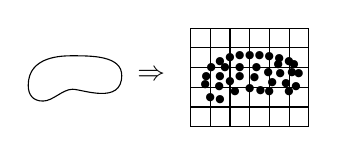
\begin{tikzpicture}[scale=0.25]
  % \draw[step=1.0,black,thin] (-3.,-1.) grid (3,4.);
  % \draw (-3,-1) -- (3,-1) -- (3,4) -- (-3,4) -- (-3,-1);
  \begin{scope}[scale=0.5]
    \draw (-3,0.6) .. controls +(1,0) and +(-1,0) .. (0,1.8)  
    .. controls +(1,0) and +(0,-3) .. (5,3.2) 
    .. controls +(0,2) and +(2,0)  .. (0,5.2) 
    .. controls +(-1,0) and +(0,3) .. (-4.5,2.2) 
    .. controls +(0,-1) and +(-1,0).. (-3,0.6) ;
    \begin{scope}  % pour limiter la portée du clip
      \clip (-3,0.6) .. controls +(1,0) and +(-1,0) .. (0,1.8) 
      .. controls +(1,0) and +(0,-3) .. (5,3.2)
      .. controls +(0,2) and +(2,0)  .. (0,5.2)
      .. controls +(-1,0) and +(0,3) .. (-4.5,2.2)
      .. controls +(0,-1) and +(-1,0).. (-3,0.6);
    \end{scope}
    %\node[below] at (0,1) {$\Omega$};
  \end{scope}
  \node at (4.,1.62) {$\Rightarrow$};
  \begin{scope}[shift={(9,0)}]
    \draw[step=1.0,black,thin] (-3.,-1.) grid (3,4.);
    % contour
    \node at (0,0.9) {\scriptsize$\bullet$}  ;
    \node at (2.5,1.65) {\scriptsize$\bullet$}  ; 
    \node at (0,2.6) {\scriptsize$\bullet$}  ;
    \node at (-2.25,1.1) {\scriptsize$\bullet$}  ; 
    \node at (-1.5,0.35) {\scriptsize$\bullet$}  ; 
    \node at (-2.,0.45) {\scriptsize$\bullet$} ;
    \node at (-2.2,1.5) {\scriptsize$\bullet$}  ; 
    \node at (-1.5,2.3) {\scriptsize$\bullet$} ; 
    \node at (2.35,1.) {\scriptsize$\bullet$}  ;
    \node at (2.25,2.15) {\scriptsize$\bullet$}  ;
    \node at (0.55,0.8) {\scriptsize$\bullet$}  ; 
    \node at (-0.5,2.6) {\scriptsize$\bullet$};
    \node at (0.5,2.59) {\scriptsize$\bullet$}  ;
    \node at (1.5,2.45) {\scriptsize$\bullet$}  ;
    \node at (1,0.75) {\scriptsize$\bullet$}; 
    \node at (2,0.75) {\scriptsize$\bullet$}  ;
    \node at (2,2.3) {\scriptsize$\bullet$}  ;
    \node at (1,2.55) {\scriptsize$\bullet$}  ;
    \node at (-1,2.5) {\scriptsize$\bullet$}  ; 
    \node at (-1.95,2.) {\scriptsize$\bullet$}  ;
    % interior
    \node at (-1.5,1.5) {\scriptsize$\bullet$}  ; 
    \node at (-1.25,2.) {\scriptsize$\bullet$}  ;
    \node at (-0.75,0.75) {\scriptsize$\bullet$}  ; 
    \node at (-1.55,1.){\scriptsize$\bullet$} ;
    \node at (-0.5,1.5) {\scriptsize$\bullet$}  ; 
    \node at (-0.5,2.) {\scriptsize$\bullet$}  ;
    \node at (0.25,1.45) {\scriptsize$\bullet$}  ;
    \node at (0.35,2.) {\scriptsize$\bullet$}  ;
    \node at (0.95,1.75) {\scriptsize$\bullet$}  ;
    \node at (1.15,1.2) {\scriptsize$\bullet$} ;
    \node at (1.45,2.15) {\scriptsize$\bullet$}  ; 
    \node at (1.55,1.65) {\scriptsize$\bullet$}  ;
    \node at (1.85,1.15) {\scriptsize$\bullet$}  ; 
    \node at (2.15,1.75) {\scriptsize$\bullet$}  ;
    \node at (-1.,1.25) {\scriptsize$\bullet$}  ;
    % \draw(3,0.5) -- (3.4,0.5) node [right]  {$\Omega_g$};
  \end{scope}
\end{tikzpicture}

%%% Local Variables:
%%% mode: latex
%%% TeX-master: "../presentation"
%%% End:
}
  {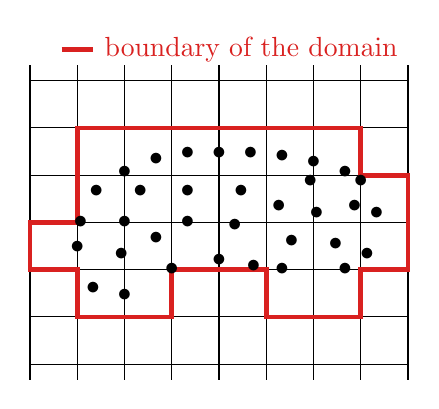
\begin{tikzpicture}[scale=0.8]
  \draw[step=.75,black,thin] (-3.,-1.) grid (3,4.);
  \draw[line width=0.6mm,Red] (-2.25,2.25) -- (-2.25,2.25)-- (-2.25,3)-- (2.25,3) --(2.25,2.25) -- (3.,2.25)-- (3.,0.75) --(2.25,0.75) --(2.25,0.) -- (0.75,0.) --(0.75,0.75) --(-0.75,0.75)-- (-0.75,0.)-- (-2.25,0.) -- (-2.25,0.75) --  (-3.,0.75)--(-3.,1.5) --(-2.25,1.5)--(-2.25,2.25);
  % contour
  \node at (0,0.9) {$\bullet$}  ; \node at (2.5,1.65) {$\bullet$}  ; 
  \node at (0,2.6) {$\bullet$}  ;\node at (-2.25,1.1) {$\bullet$}  ; 
  \node at (-1.5,0.35) {$\bullet$}  ; \node at (-2.,0.45) {$\bullet$}  ;
  \node at (-2.2,1.5) {$\bullet$}  ; \node at (-1.5,2.3) {$\bullet$}  ; 
  \node at (2.35,1.) {$\bullet$}  ; \node at (2.25,2.15) {$\bullet$}  ;
  \node at (0.55,0.8) {$\bullet$}  ; \node at (-0.5,2.6) {$\bullet$}  ; 
  \node at (0.5,2.59) {$\bullet$}  ; \node at (1.5,2.45) {$\bullet$}  ;
  \node at (1,0.75) {$\bullet$}; \node at (2,0.75) {$\bullet$}  ;
  \node at (2,2.3) {$\bullet$}  ; \node at (1,2.55) {$\bullet$}  ;
  \node at (-1,2.5) {$\bullet$}  ; \node at (-1.95,2.) {$\bullet$}  ;
  % interior
  \node at (-1.5,1.5) {$\bullet$}  ; \node at (-1.25,2.) {$\bullet$}  ;
  \node at (-0.75,0.75) {$\bullet$}  ; \node at (-1.55,1.) {$\bullet$}  ;
  \node at (-0.5,1.5) {$\bullet$}  ; \node at (-0.5,2.) {$\bullet$}  ;
  \node at (0.25,1.45) {$\bullet$}  ; \node at (0.35,2.) {$\bullet$}  ;
  \node at (0.95,1.75) {$\bullet$}  ; \node at (1.15,1.2) {$\bullet$}  ;
  \node at (1.45,2.15) {$\bullet$}  ; \node at (1.55,1.65) {$\bullet$}  ;
  \node at (1.85,1.15) {$\bullet$}  ; \node at (2.15,1.75) {$\bullet$}  ;
  \node at (-1.,1.25) {$\bullet$}  ;
  \draw[line width=0.6mm,Red] (-2.5,4.25) -- (-2.,4.25) node [right] {\text{boundary of the domain}};
\end{tikzpicture}}
  \caption{Representation of a continuum body by a set of material points in $\Rbb^2$.}
  \label{fig:domain}	
\end{figure}
Analogously to the Finite Element Method (FEM) \cite{Belytschko}, the velocity is approximated on the MPM background mesh by:
\begin{equation}
  \label{eq:approximation_basis}
  \vect{v}(\vect{x},t)=S_j(\vect{x})\vect{v}^{j}(t)
\end{equation}
where $\vect{v}^{i}$ is the velocity of the $i$th grid node, and $S_i(\vect{x})$ the (linear) shape function attached to it. One feature of the MPM is that the mass density is approximated in the grid based on the mass carried by each material point:
\begin{equation}
  \label{eq:density_approx}
  \rho\(\vect{x},t\)=\sum_{p=1}^{N_p} m_p \: \delta(\vect{\phi}(\vect{X}^p,t)-\vect{x})=\sum_{p=1}^{N_p} m_p \: \delta(\vect{x}^p-\vect{x})
\end{equation}
where the delta Dirac distribution $\delta$ is often referred to as the \textit{characteristic function} of material points, and $\vect{x}^p$ is the position of the $p$th particle. In what follows, the dependence on time will be omitted for simplicity and $p$ and $(i,j)$ stand respectively for material points and nodes. 

By introducing successively in the weak form \eqref{eq:linear_momentum_weak_form} the specific Cauchy tensor $\rho \tens{\bar{\sigma}}=\tens{\sigma}$ and the approximation of mass density \eqref{eq:density_approx}, the integration property of the delta Dirac distribution allows to write:
\begin{equation}
  \begin{aligned}
    &\text{Find $\vect{v}\in \Vscr_h^1$ such that} \\
    & \sum_{p=1}^{N_p} m_p  \[\vect{\dot{v}}(\vect{x}^p) \cdot \vect{w}(\vect{x}^p) + \tens{\bar{\sigma}}(\vect{x}^p):\nablat \vect{w}(\vect{x}^p) \]  = \sum_{p=1}^{N_p}m_p \vect{b}(\vect{x}^p)\cdot \vect{w}(\vect{x}^p) + \int_{\partial \Omega^\sigma_t} \vect{T}_d\cdot\vect{w}\: ds  \qquad \forall \: \vect{w} \in \Vscr_{h,0}^1, \forall\: t \in \tau
  \end{aligned}
\end{equation}
Then, with the finite element approximation \eqref{eq:approximation_basis}, the weak form reads:
\begin{equation}
  \label{eq:mpm_discrete_weak}
    \begin{aligned}
      &\text{Find $\vect{v} \in \Vscr_h^1$ such that} \\
      & \vect{w}^i \sum_{p=1}^{N_p} m_p  \[ S_{ip} S_{jp} \vect{\dot{v}}^j + \nablav S_{ip} \cdot \tens{\bar{\sigma}}^p \]  =  \vect{w}^i\( \sum_{p=1}^{N_p}m_p S_{ip}\vect{b}^p  + \int_{\partial \Omega^\sigma_t} S_i(\vect{x})\vect{T}_d\: ds\)  \qquad \forall \: \vect{w} \in \Vscr_{h,0}^1, \forall \: t \in \tau
  \end{aligned}
\end{equation}
in which $S_{ip}=S_i(\vect{x}^p)$ and $\tens{\bar{\sigma}}^p=\tens{\bar{\sigma}}(\vect{x}^p)$. Next, the arbitrariness of the test function $\vect{w}$ leads to the semi-discrete equation in matrix form:
\begin{equation}
  \label{eq:mpm_semi-discrete}
  M_{ij} \vect{\dot{v}}^j = \vect{f}_{int}^i + \vect{f}_{ext}^i 
\end{equation}
where the definition of the mass matrix $M_{ij}$ and internal and external force vectors $\vect{f}_{int}^i $ and $\vect{f}_{ext}^i$ are:
\begin{subequations}
  \begin{alignat}{1}
    & M_{ij}= \sum_{p=1}^{N_p} m_p  S_{ip} S_{jp} \label{eq:mass_matrix}\\
    & \vect{f}_{int}^i = - \sum_{p=1}^{N_p} m_p \nablav S_{ip} \cdot \tens{\bar{\sigma}}^p \label{eq:int_forces}\\
    & \vect{f}_{ext}^i =\sum_{p=1}^{N_p}m_p S_{ip}\vect{b}^p  + \int_{\partial \Omega^\sigma_t} S_i(\vect{x})\vect{T}_d\: ds \label{eq:ext_forces}
  \end{alignat}
\end{subequations}
In addition, note that particles play the role of integration points in the semi-discrete form so that the mass matrix depends on the positions of material points in the grid and must be computed at each time step. Hence, the MPM can be seen as an extension of FEM with moving Gauss points. However, this quadrature rule results in a consistent mass matrix $M_{ji}$ that may be singular when only one material point lies in an element due to reduced integration. The use of a linear combination of the (positive-definite) diagonally lumped mass matrix $M^L_i=\sum_p S_{ip}m_p$, and the (positive semi-definite) consistent mass matrix is then recommended \cite{Love}. Nevertheless, since no parameter values are prescribed for this combination, the lumped mass matrix is widely used in MPM simulations in spite of additional dissipation of kinetic energy it introduces \cite{Mass_Flip}. 

At last, system \eqref{eq:mpm_semi-discrete} is solved for nodal accelerations $\vect{\dot{v}}^i$, from which time integration allows to update nodal velocities. Hence, the time interval $\tau$ is discretized in $N_T$ sub-intervals of size $\Delta t^n$ such that $\sum_{n=1}^{N_T} \Delta t^n = T$ and time integration is performed with an explicit forward Euler algorithm. The discrete equations are thus written:
\begin{equation}
  \label{eq:mpm_discrete}
  \frac{\vect{v}^{i,n+1}-\vect{v}^{i,n}}{\Delta t^n} = \vect{\dot{v}}^i
\end{equation}
where the superscripts $\bullet^{k,l}$ denote the time step $l$ at which the $k$th nodal field is evaluated. 

Recall that the background grid inherited from FLIP is arbitrary so that fields must be projected between particles and nodes to $(i)$ solve the linear system \eqref{eq:mpm_semi-discrete} and $(ii)$ advect the solution by moving material points. The first mapping step, required to build the discrete form, aims at satisfying the conservation of linear momentum:
\begin{equation}
  \label{eq:particles2nodes}
  M^{L,n}_i \vect{v}^{i,n} = \sum_{p=1}^{N_p} S_{ip}m_p \vect{v}^{p,n}
\end{equation}
that must be solved for every $\vect{v}^i$. Once the nodal accelerations are calculated from system \eqref{eq:mpm_semi-discrete}, nodale velocity increments can be computed to \textbf{update} the velocity of each material point by following FLIP approach \cite{PIC_Nishiguchi}:
%the velocity of each material points is \textbf{updated} according to the approach followed in FLIP \cite{PIC_Nishiguchi}:
\begin{equation}
  \label{eq:mp_velocity_update}
  \vect{v}^{p,n+1}= \vect{v}^{p,n}+ \Delta t^n \sum_{i=1}^{N_n} S_{ip}\vect{\dot{v}}^{i}
\end{equation}
On the other hand, updated nodal velocities resulting from the solution of \eqref{eq:mpm_discrete} are used to update the particles positions:
\begin{equation}
  \label{eq:position_update}
  \vect{x}^{p,n+1}=\vect{x}^{p,n} + \Delta t^n\sum_{i=1}^{N_n} S_{ip}\vect{v}^{i,n+1} 
\end{equation}

\begin{remark}
  \label{rq:dual_velo}
  Equations \eqref{eq:mp_velocity_update} and \eqref{eq:position_update} lead to a double definition of the velocity since the time derivative of the displacement of a given particle does not correspond to its velocity. This can be seen in a finite differences sense by combining equations \eqref{eq:position_update} and \eqref{eq:mpm_discrete}:
  \begin{equation}
    \label{eq:double_velocity_mpm}
    \frac{\vect{x}^{p,n+1} - \vect{x}^{p,n}}{\Delta t^n}  =\sum_{i=1}^{N_n} S_{ip}\vect{v}^{i,n+1} = \sum_{i=1}^{N_n} S_{ip} \( \vect{v}^{i,n} + \Delta t \vect{\dot{v}}^i\)
  \end{equation}
  Next, on gets from equation \eqref{eq:mp_velocity_update}:
  \begin{equation*}
    \Delta t^n \sum_{i=1}^{N_n} S_{ip}\vect{\dot{v}}^{i}= \vect{v}^{p,n+1}- \vect{v}^{p,n}
  \end{equation*}
  which, once introduced in \eqref{eq:double_velocity_mpm}, yields:
  \begin{equation}
    \frac{\vect{x}^{p,n+1} - \vect{x}^{p,n}}{\Delta t^n}= \sum_{i=1}^{N_n} S_{ip} \vect{v}^{i,n} +   \vect{v}^{p,n+1} - \vect{v}^{p,n}
  \end{equation}
  Considering the mapping \eqref{eq:particles2nodes}, the right-hand side of this equation does not identify to the updated material point velocity, it then comes out that $\vect{\dot{x}}^{p,n+1} \ne \vect{v}^{p,n+1}$. 
\end{remark}

The computation of constitutive equations is performed at material points within the MPM, thanks to the updated nodal velocity field and the gradient of shape functions. One has therefore some freedom since stress can be updated right after either the resolution of \eqref{eq:mpm_discrete} or the projection \eqref{eq:particles2nodes}. The first option yields the \textit{Update Stress Last} (USL) algorithm while the second implementation is called \textit{Update Stress First} (USF) \cite{Bardenhagen_USF_USL}. 

\subsubsection{Boundary conditions enforcement}

Writing the weak form of linear momentum balance on the grid implies that Neumann boundary conditions are enforced on nodes through the external force vector \eqref{eq:ext_forces}. Next, since stress are computed at material points based the nodal velocity field, Dirichlet boundary conditions are also dealt with at nodes. For USL, it is done once the solution is updated on the grid so that stresses can be computed and material points kinematic can be updated. On the other hand, USF formulation  first requires applying Dirichlet boundary conditions to compute the stress, and then again after solving discrete equations for particles kinematic \cite{USF_USL}. Furthermore, the enforcement of boundary condition is still a challenging aspect of the material point method (as others mesh-free methods) for problems involving complex geometries, see for instance \cite{Bcs_MPM}.

\subsubsection{Solution scheme summary}
All the ingredients derived above are now summarized to write the procedure followed within the MPM for one time step. Position and velocity vectors $\vect{x}^n$ and $\vect{v}^n$ are supposed known at every material points that discretize the continuum body in a computational grid at time $t^n$. USL formulation further requires the knowledge of the specific stress tensor $\tens{\bar{\sigma}}^n$ at material points. The MPM solution scheme then consists of the following steps:
\begin{itemize}
\item[(a)] Computation of the consistent and lumped mass matrices as well as external forces (Neumann boundary conditions) from equations \eqref{eq:mass_matrix} and \eqref{eq:ext_forces}.
\item[(b)] Projection of fields to the grid \eqref{eq:particles2nodes} and enforce Dirichlet boundary conditions on the nodal velocity. 
$\newline$
\textbf{USF formulation:} enforcement of Dirichlet boundary conditions on the mesh and integration of constitutive equations.
\item[(c)] Evaluation of internal forces from equation \eqref{eq:int_forces}.
\item[(d)] Solution of the semi-discrete and discrete forms \eqref{eq:mpm_semi-discrete} and \eqref{eq:mpm_discrete} so that nodal accelerations $\vect{\dot{v}}^i$ and updated velocities $\vect{v}^{i,n+1}$ are determined. Enforcement of Dirichlet boundary conditions.%: set the velocity of boundary nodes to the prescribed values and their accelerations to zero.
\item[(e)] Update material points velocities and positions with equations \eqref{eq:mp_velocity_update} and \eqref{eq:position_update} respectively. At this point the mesh has virtually moved, but since fields have been transferred back to particles, the underlying grid can be discarded and rebuilt for computational convenience, thus involving the projection (b) at the subsequent time increment. 
$\newline$
\textbf{USL formulation:} computation of constitutive equations.
%\item[(f)] If the USL implementation is set, constitutive equations must be integrated.
\end{itemize}

Although the material point method presented above has been successfully applied to a wide range of complex engineering problems involving finite deformations \cite{Wieckowski}, this approach suffers from limitations which are discussed in the next section. 
\subsection{Lagrangian formulation of the MPM}
Despite the above Eulerian formulation of the MPM is widely used, an alternative method that solves a discrete system on a reference configuration and which derivation is briefly recalled here, has also been developed \cite{Love}.

Though an Eulerian equation is solved, the fact of using moving material points to store and carry the fields confers the method a Lagrangian nature.
\subsubsection*{Discrete equations}
An approximate solution of the conservation of Lagrangian linear momentum is seeked within the time interval $\tau=\[0,T\]$, in a solid with volume $\Omega_0$ and boundary $\partial \Omega_0$ in the reference configuration. The body is subject to traction forces and prescribed velocity on its boundaries:
\begin{align}
  & \tens{\Pi}\cdot\vect{N}=\vect{T}_d \quad \text{on } \partial \Omega_0^\Pi\\
  & \vect{v} = \vect{\tilde{v}} \quad \text{on } \partial \Omega_0^v
\end{align}
where $\vect{N}$ is the outward normal vector to $\partial \Omega_0$ and the set of boundaries satisfies $\partial \Omega_0 =\partial \Omega^\Pi_0 \cap \partial \Omega^v_0$. Thus, the weak form of the balance equation of Lagrangian linear momentum \eqref{eq:Lagrangian_linear_momentum} is written in the reference configuration by means of the Galerkin approach. After integration by parts, one gets:
\begin{equation}
  \label{eq:lagrangian_momentum_weak_form}
  \begin{aligned}
    &\text{Find $\vect{v}\in \Vscr_h^1$ such that} \\
    &\int_{\Omega_0}  \rho_0  \vect{\dot{v}} \cdot \vect{w}\: dv + \int_{\Omega_0}\tens{\Pi}: 
    \nablat_0 \vect{w} \:dv - \int_{\partial \Omega^\Pi_0} \vect{T}_d\cdot\vect{w}\: ds= \int_{\Omega_0} \rho_0 \vect{b}\cdot \vect{w} \: dv  \qquad \forall \: \vect{w} \in \Vscr_{h,0}^1, \forall\: t \in \tau
  \end{aligned}
\end{equation}
Representing the solid in the reference configuration with a collection of $N_p$ material points that can move in an arbitrary grid.
Similarly to the Eulerian formulation, the reference mass density is defined based on the masses carried by the particles and the delta Dirac distribution: $\rho_0(\vect{X})=\sum_{p=1}^{N_p}m_p \delta\(\vect{X}^p-\vect{X}\)$. Thus, the specific PK1 stress tensor $\rho_0\tens{\bar{\Pi}}=\tens{\Pi}$ is introduced so that volume integrals of the weak are evaluated by treating particles as quadrature points:
\begin{equation}
  \label{eq:discrete_lagrangian_momentum_weak_form}
  \begin{aligned}
    &\text{Find $\vect{v}\in \Vscr_h^1$ such that} \\
    & \sum_{p=1}^{N_p}  m_p\( \vect{\dot{v}}^p \cdot \vect{w}^p + \tens{\bar{\Pi}}^p:
    \nablat_0 \vect{w}^p \) - \int_{\partial \Omega^\Pi_0} \vect{T}_d\cdot\vect{w}\: ds= \sum_{p=1}^{N_p} m_p \vect{b}^p\cdot \vect{w}^p   \qquad \forall \: \vect{w} \in \Vscr_{h,0}^1, \forall\: t \in \tau
  \end{aligned}
\end{equation}
%Note that in equation \eqref{eq:discrete_lagrangian_momentum_weak_form}, the superscipt $p$ denotes a field evaluated at the $p$th material point position in the reference configuration.
At last, shape functions defined at nodes of the grid, combined with the arbitrariness of the test field $\vect{w}$, lead to the semi-discrete form:
\begin{equation}
  \label{eq:lagrangian_mpm_semi-discrete}
  M_{ij} \vect{\dot{v}}^j = \vect{f}_{int}^i + \vect{f}_{ext}^i 
\end{equation}
with the following definitions of the mass matrix and internal and external force vectors:
\begin{subequations}
  \begin{alignat}{1}
    & M_{ij}= \sum_{p=1}^{N_p} m_p  S_{ip} S_{jp}\\
    & \vect{f}_{int}^i = - \sum_{p=1}^{N_p} m_p \nablav_0 S_{ip} \cdot \tens{\bar{\Pi}}^p\\
    & \vect{f}_{ext}^i =\sum_{p=1}^{N_p}m_p S_{ip}\vect{b}^p  + \int_{\partial \Omega^\sigma_t} S_i(\vect{x})\vect{T}_d\: ds 
  \end{alignat}
\end{subequations}

\begin{remark}
  The description of the reference mass density used yields a discrete weak form \eqref{eq:discrete_lagrangian_momentum_weak_form} in which fields are evaluated at the positions of material points \textbf{in the reference configuration}, namely for instance: $\vect{v}^p=\vect{v}(\vect{X}^p)$. As a consequence, the shape functions and the gradient of shape functions are also evaluated in the reference configuration.
\end{remark}

\subsubsection*{Solution scheme}
Actualisation du gradient de la tranformation et de la fonction transformation. Résoudre sur la configuration précédente et non nécessairement de référence.
\subsection{Shortcomings of the MPM}

\subsubsection*{The grid-crossing instability}
The research on MPM mainly focused so far on the instability arising from the computation of internal forces when material points move from one cell to another, the so-called \textit{grid-crossing} error \cite{Gimp}. In that case, the discontinuity of the gradient of shape functions across element interfaces yields tremendous noise in the numerical solution. The \textbf{Generalized Interpolation Material Point Method} (GIMP) addressed this issue by modifying the particles characteristic function, thus widening the domain of influence of material points \cite{Gimp}. By doing so, every particles are given a domain having a constant shape or not, that must be tracked during the computation, leading respectively to the uniform GIMP (uGIMP) or contiguous particle GIMP (cpGIMP) formulations \cite{Book_MPM}. In the cpGIMP algorithm, diagonal entries of the deformation gradient are used to update the "shapes" of particles. The \textbf{Convected Particle Domain Interpolation} (CPDI) \cite{CPDI}, on the other hand, accounts for shear deformations and rotations of particles domains, thus providing an improvement of GIMP. However, those methods involve other difficulties related to the tracking of the deforming domains of material points in the Eulerian grid, and may also suffer from mesh entanglement \cite{DDMPM0}. Other approaches consisting in the direct modification of the approximation basis have then been followed to tackle the grid-crossing error. First, the \textbf{B-Spline Material Point Method} (BSMPM) \cite{Steffen_quadError} uses quadratic or cubic B-Spline functions with continuous gradients as nodal shape functions allowing to circumvent the instability \cite{MPM_BSpline1}. % (which can be seen as an IsoGeometric Analysis IGA \cite{IGA_Hughes} for immersed boundary problems, notion of unification ? c'est plus pour du fluide structure cette terminologie)
Second, the classical approximation basis is used and modified gradients with extended supports are introduced in the \textbf{Dual Domain Material Point Method} (DDMPM) \cite{DDMPM0}. BSMPM and DDMPM  both solve the grid-crossing error by widening the domain of influence of material points since B-Spline functions span more cells than Lagrange polynomials, and the support of the modified gradient of DDMPM is larger than that of the shape functions.  

\subsubsection*{The back-mapping instability}
Numerical oscillations appear in the MPM solution even for problems that do not involve the grid-crossing instability, that is due to the updating of the velocity field at material points \cite{Mass_Flip}. As an illustration, consider a one-dimensional elastic bar of length $L=6\:m$ with Young's modulus $E=200 \:GPa$ and mass density $\rho=7800 \:kg\cdot m^{-3}$ within the infinitesimal theory. The bar is initially in a free stress state and Riemann-type initial velocities are prescribed along the bar, that is: $v=v_0>0$ for $x\in[0,L/2[$ and $v=-v_0$ for $x \in ]L/2,L]$.
\begin{figure}[ht]
  \centering
  {\definecolor{Purple}{RGB}{120,28,129}
\definecolor{Orange}{RGB}{231,133,50}
\definecolor{Blue}{RGB}{63,96,174}
\definecolor{Red}{RGB}{217,33,32}
\definecolor{Duck}{RGB}{83,158,182}
\definecolor{Green}{RGB}{109,179,136}
\definecolor{Yellow}{RGB}{202,184,67}
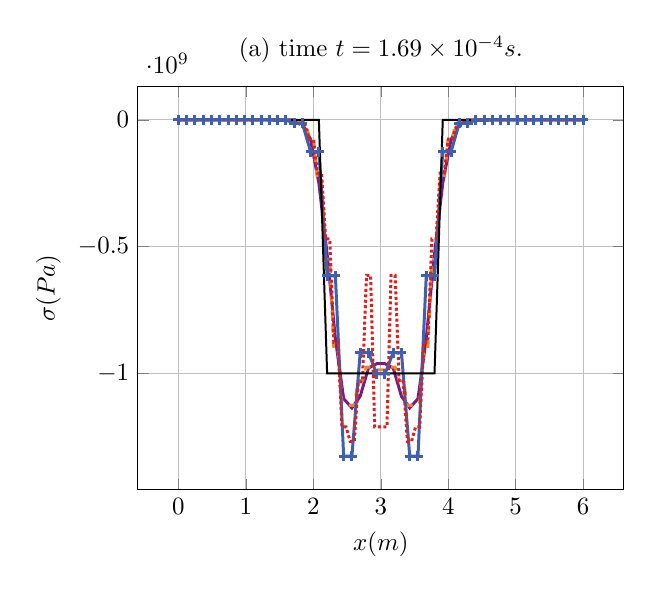
\begin{tikzpicture}[scale=0.9]
\begin{axis}[xlabel=$x (m)$,ylabel=$\sigma (Pa)$,ymajorgrids=true,xmajorgrids=true,title={(a) time $t =1.69\times 10^{-4}s.$}]
\addplot[Purple,very thick,mark=none,solid] coordinates {(0.0,-9.62200780097e-08) (0.122448979592,-1.92440156019e-07) (0.244897959184,-9.62200780097e-08) (0.367346938776,0.0) (0.489795918367,9.62200780097e-08) (0.612244897959,-9.62200780097e-08) (0.734693877551,-1.92440156019e-07) (0.857142857143,-9.62200780097e-08) (0.979591836735,-9.62200780097e-08) (1.10204081633,0.0) (1.22448979592,9.62200780097e-08) (1.34693877551,-9.62200780097e-08) (1.4693877551,0.0) (1.59183673469,0.0) (1.71428571429,0.0) (1.83673469388,-15437652.4848) (1.95918367347,-78183137.9185) (2.08163265306,-249067223.585) (2.20408163265,-529536815.675) (2.32653061224,-862202048.46) (2.44897959184,-1099498863.41) (2.57142857143,-1135789315.44) (2.69387755102,-1090007223.73) (2.81632653061,-978780358.738) (2.9387755102,-961497360.562) (3.0612244898,-961497360.562) (3.18367346939,-978780358.738) (3.30612244898,-1090007223.73) (3.42857142857,-1135789315.44) (3.55102040816,-1099498863.41) (3.67346938776,-862202048.46) (3.79591836735,-529536815.675) (3.91836734694,-249067223.585) (4.04081632653,-78183137.9185) (4.16326530612,-15437652.4848) (4.28571428571,-3.85185988877e-23) (4.40816326531,-9.62200780097e-08) (4.5306122449,9.62200780097e-08) (4.65306122449,9.62200780097e-08) (4.77551020408,9.62200780097e-08) (4.89795918367,-2.88660234029e-07) (5.02040816327,-9.62200780097e-08) (5.14285714286,9.62200780097e-08) (5.26530612245,1.92440156019e-07) (5.38775510204,2.88660234029e-07) (5.51020408163,9.62200780097e-08) (5.63265306122,0.0) (5.75510204082,0.0) (5.87755102041,0.0) (6.0,-9.62200780097e-08) };
\addplot[Orange,very thick,mark=none,dashed] coordinates {(0.0,0.0) (0.0606060606061,0.0) (0.121212121212,9.52481580298e-08) (0.181818181818,9.52481580298e-08) (0.242424242424,9.52481580298e-08) (0.30303030303,9.52481580298e-08) (0.363636363636,0.0) (0.424242424242,0.0) (0.484848484848,-9.52481580298e-08) (0.545454545455,-9.52481580298e-08) (0.606060606061,-1.9049631606e-07) (0.666666666667,-1.9049631606e-07) (0.727272727273,0.0) (0.787878787879,0.0) (0.848484848485,0.0) (0.909090909091,0.0) (0.969696969697,-3.85185988877e-23) (1.0303030303,-3.85185988877e-23) (1.09090909091,-9.52481580298e-08) (1.15151515152,-9.52481580298e-08) (1.21212121212,9.52481580298e-08) (1.27272727273,9.52481580298e-08) (1.33333333333,9.52481580298e-08) (1.39393939394,9.52481580298e-08) (1.45454545455,-1.9049631606e-07) (1.51515151515,-1.9049631606e-07) (1.57575757576,1.9049631606e-07) (1.63636363636,1.9049631606e-07) (1.69696969697,0.0) (1.75757575758,0.0) (1.81818181818,-9533923.2537) (1.87878787879,-9533923.2537) (1.93939393939,-67166647.336) (2.0,-67166647.336) (2.06060606061,-239339979.822) (2.12121212121,-239339979.822) (2.18181818182,-549695480.518) (2.24242424242,-549695480.518) (2.30303030303,-900240202.504) (2.36363636364,-900240202.504) (2.42424242424,-1118552245.0) (2.48484848485,-1118552245.0) (2.54545454545,-1125362633.2) (2.60606060606,-1125362633.2) (2.66666666667,-1028724363.35) (2.72727272727,-1028724363.35) (2.78787878788,-975375246.836) (2.84848484848,-975375246.836) (2.90909090909,-986009278.185) (2.9696969697,-986009278.185) (3.0303030303,-986009278.185) (3.09090909091,-986009278.185) (3.15151515152,-975375246.836) (3.21212121212,-975375246.836) (3.27272727273,-1028724363.35) (3.33333333333,-1028724363.35) (3.39393939394,-1125362633.2) (3.45454545455,-1125362633.2) (3.51515151515,-1118552245.0) (3.57575757576,-1118552245.0) (3.63636363636,-900240202.504) (3.69696969697,-900240202.504) (3.75757575758,-549695480.518) (3.81818181818,-549695480.518) (3.87878787879,-239339979.822) (3.93939393939,-239339979.822) (4.0,-67166647.336) (4.06060606061,-67166647.336) (4.12121212121,-9533923.2537) (4.18181818182,-9533923.2537) (4.24242424242,9.52481580298e-08) (4.30303030303,9.52481580298e-08) (4.36363636364,-9.52481580298e-08) (4.42424242424,-9.52481580298e-08) (4.48484848485,0.0) (4.54545454545,0.0) (4.60606060606,0.0) (4.66666666667,0.0) (4.72727272727,0.0) (4.78787878788,0.0) (4.84848484848,0.0) (4.90909090909,0.0) (4.9696969697,0.0) (5.0303030303,0.0) (5.09090909091,0.0) (5.15151515152,0.0) (5.21212121212,0.0) (5.27272727273,0.0) (5.33333333333,0.0) (5.39393939394,0.0) (5.45454545455,0.0) (5.51515151515,0.0) (5.57575757576,0.0) (5.63636363636,0.0) (5.69696969697,0.0) (5.75757575758,0.0) (5.81818181818,0.0) (5.87878787879,0.0) (5.93939393939,9.52481580298e-08) (6.0,9.52481580298e-08) };
\addplot[Blue,very thick,mark=+,solid] coordinates {(0.0,-3.84880312039e-07) (0.122448979592,2.88660234029e-07) (0.244897959184,-5.77320468058e-07) (0.367346938776,2.88660234029e-07) (0.489795918367,-9.62200780097e-08) (0.612244897959,2.88660234029e-07) (0.734693877551,-4.3483336004) (0.857142857143,-4.34833340796) (0.979591836735,-560.668787915) (1.10204081633,-560.668788299) (1.22448979592,-29850.7439455) (1.34693877551,-29850.7439456) (1.4693877551,-846060.279927) (1.59183673469,-846060.279927) (1.71428571429,-13703737.6015) (1.83673469388,-13703737.6015) (1.95918367347,-126206739.753) (2.08163265306,-126206739.753) (2.20408163265,-614922268.389) (2.32653061224,-614922268.389) (2.44897959184,-1325731906.52) (2.57142857143,-1325731906.52) (2.69387755102,-917663590.795) (2.81632653061,-917663590.795) (2.9387755102,-1001790561.8) (3.0612244898,-1001790561.8) (3.18367346939,-917663590.795) (3.30612244898,-917663590.795) (3.42857142857,-1325731906.52) (3.55102040816,-1325731906.52) (3.67346938776,-614922268.389) (3.79591836735,-614922268.389) (3.91836734694,-126206739.753) (4.04081632653,-126206739.753) (4.16326530612,-13703737.6015) (4.28571428571,-13703737.6015) (4.40816326531,-846060.279927) (4.5306122449,-846060.279927) (4.65306122449,-29850.7439458) (4.77551020408,-29850.7439452) (4.89795918367,-560.668787818) (5.02040816327,-560.668788011) (5.14285714286,-4.34833331174) (5.26530612245,-4.34833340796) (5.38775510204,1.92440156019e-07) (5.51020408163,-9.62200780097e-08) (5.63265306122,1.92440156019e-07) (5.75510204082,-2.88660234029e-07) (5.87755102041,4.81100390048e-07) (6.0,-2.88660234029e-07) };
\addplot[Red,very thick,mark=none,densely dotted] coordinates {(0.0,0.0) (0.0606060606061,0.0) (0.121212121212,9.52481580298e-08) (0.181818181818,9.52481580298e-08) (0.242424242424,-7.70371977755e-23) (0.30303030303,-7.70371977755e-23) (0.363636363636,-9.52481580298e-08) (0.424242424242,-9.52481580298e-08) (0.484848484848,-1.9049631606e-07) (0.545454545455,-1.9049631606e-07) (0.606060606061,1.9049631606e-07) (0.666666666667,1.9049631606e-07) (0.727272727273,-0.326493160065) (0.787878787879,-0.326493160065) (0.848484848485,-4.24441250957) (0.909090909091,-4.24441250957) (0.969696969697,-75.0667952395) (1.0303030303,-75.0667952395) (1.09090909091,-676.110516968) (1.15151515152,-676.110516968) (1.21212121212,-6409.50756423) (1.27272727273,-6409.50756423) (1.33333333333,-42608.4474487) (1.39393939394,-42608.4474487) (1.45454545455,-271096.202803) (1.51515151515,-271096.202803) (1.57575757576,-1361323.47494) (1.63636363636,-1361323.47494) (1.69696969697,-6186277.73843) (1.75757575758,-6186277.73843) (1.81818181818,-23394049.9045) (1.87878787879,-23394049.9045) (1.93939393939,-76154273.8888) (2.0,-76154273.8888) (2.06060606061,-210327688.316) (2.12121212121,-210327688.316) (2.18181818182,-469773248.386) (2.24242424242,-469773248.386) (2.30303030303,-877374801.132) (2.36363636364,-877374801.132) (2.42424242424,-1211041212.86) (2.48484848485,-1211041212.86) (2.54545454545,-1267995558.57) (2.60606060606,-1267995558.57) (2.66666666667,-1032834595.27) (2.72727272727,-1032834595.27) (2.78787878788,-612908579.142) (2.84848484848,-612908579.142) (2.90909090909,-1210327521.41) (2.9696969697,-1210327521.41) (3.0303030303,-1210327521.41) (3.09090909091,-1210327521.41) (3.15151515152,-612908579.142) (3.21212121212,-612908579.142) (3.27272727273,-1032834595.27) (3.33333333333,-1032834595.27) (3.39393939394,-1267995558.57) (3.45454545455,-1267995558.57) (3.51515151515,-1211041212.86) (3.57575757576,-1211041212.86) (3.63636363636,-877374801.132) (3.69696969697,-877374801.132) (3.75757575758,-469773248.386) (3.81818181818,-469773248.386) (3.87878787879,-210327688.316) (3.93939393939,-210327688.316) (4.0,-76154273.8888) (4.06060606061,-76154273.8888) (4.12121212121,-23394049.9045) (4.18181818182,-23394049.9045) (4.24242424242,-6186277.73843) (4.30303030303,-6186277.73843) (4.36363636364,-1361323.47494) (4.42424242424,-1361323.47494) (4.48484848485,-271096.202803) (4.54545454545,-271096.202803) (4.60606060606,-42608.4474489) (4.66666666667,-42608.4474489) (4.72727272727,-6409.50756433) (4.78787878788,-6409.50756433) (4.84848484848,-676.110516873) (4.90909090909,-676.110516873) (4.9696969697,-75.0667953347) (5.0303030303,-75.0667953347) (5.09090909091,-4.24441231907) (5.15151515152,-4.24441231907) (5.21212121212,-0.326493255313) (5.27272727273,-0.326493255313) (5.33333333333,0.0) (5.39393939394,0.0) (5.45454545455,0.0) (5.51515151515,0.0) (5.57575757576,0.0) (5.63636363636,0.0) (5.69696969697,0.0) (5.75757575758,0.0) (5.81818181818,0.0) (5.87878787879,0.0) (5.93939393939,0.0) (6.0,0.0) };
\addplot[black,thick] coordinates {(0.0,-0.0) (0.122448979592,-0.0) (0.244897959184,-0.0) (0.367346938776,-0.0) (0.489795918367,-0.0) (0.612244897959,-0.0) (0.734693877551,-0.0) (0.857142857143,-0.0) (0.979591836735,-0.0) (1.10204081633,-0.0) (1.22448979592,-0.0) (1.34693877551,-0.0) (1.4693877551,-0.0) (1.59183673469,-0.0) (1.71428571429,-0.0) (1.83673469388,-0.0) (1.95918367347,-0.0) (2.08163265306,-0.0) (2.20408163265,-1000000000.0) (2.32653061224,-1000000000.0) (2.44897959184,-1000000000.0) (2.57142857143,-1000000000.0) (2.69387755102,-1000000000.0) (2.81632653061,-1000000000.0) (2.9387755102,-1000000000.0) (3.0612244898,-1000000000.0) (3.18367346939,-1000000000.0) (3.30612244898,-1000000000.0) (3.42857142857,-1000000000.0) (3.55102040816,-1000000000.0) (3.67346938776,-1000000000.0) (3.79591836735,-1000000000.0) (3.91836734694,-0.0) (4.04081632653,-0.0) (4.16326530612,-0.0) (4.28571428571,-0.0) (4.40816326531,-0.0) (4.5306122449,-0.0) (4.65306122449,-0.0) (4.77551020408,-0.0) (4.89795918367,-0.0) (5.02040816327,-0.0) (5.14285714286,-0.0) (5.26530612245,-0.0) (5.38775510204,-0.0) (5.51020408163,-0.0) (5.63265306122,-0.0) (5.75510204082,-0.0) (5.87755102041,-0.0) (6.0,-0.0) };
%\legend{USL 1ppc,USL 2ppc,USF 1ppc,USF 2ppc}
\end{axis}
\end{tikzpicture}
 \phantomsubcaption \label{subfig:US_diffusion_10}}
  {\definecolor{Purple}{RGB}{120,28,129}
\definecolor{Orange}{RGB}{231,133,50}
\definecolor{Blue}{RGB}{63,96,174}
\definecolor{Red}{RGB}{217,33,32}
\definecolor{Duck}{RGB}{83,158,182}
\definecolor{Green}{RGB}{109,179,136}
\definecolor{Yellow}{RGB}{202,184,67}
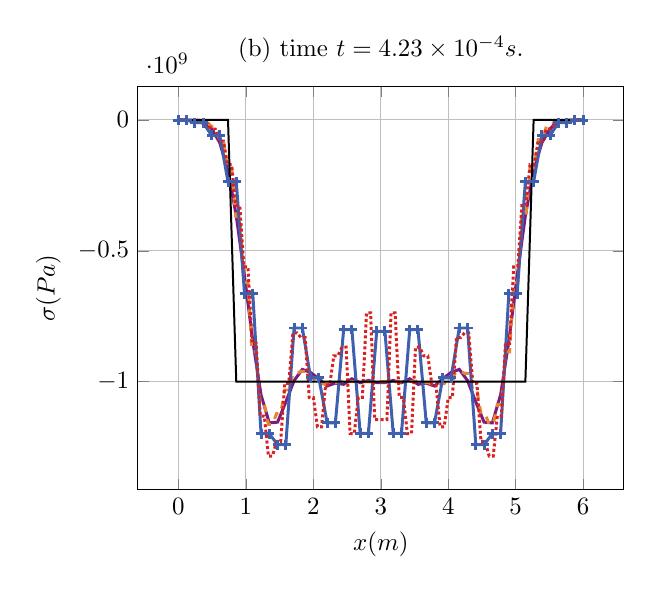
\begin{tikzpicture}[scale=0.9]
\begin{axis}[xlabel=$x (m)$,ylabel=$\sigma (Pa)$,ymajorgrids=true,xmajorgrids=true,title={(b) time $t= 4.23\times 10^{-4}s.$}]
\addplot[Purple,very thick,mark=none,solid] coordinates {(0.0,-39934.2174897) (0.122448979592,-406302.064953) (0.244897959184,-2420460.88495) (0.367346938776,-10136844.8366) (0.489795918367,-33063216.5915) (0.612244897959,-87547121.3685) (0.734693877551,-194171704.565) (0.857142857143,-366493404.576) (0.979591836735,-596875114.898) (1.10204081633,-845116689.368) (1.22448979592,-1050481005.19) (1.34693877551,-1157297307.0) (1.4693877551,-1154376682.02) (1.59183673469,-1077374033.62) (1.71428571429,-995689036.388) (1.83673469388,-952936697.469) (1.95918367347,-964832377.273) (2.08163265306,-988568067.368) (2.20408163265,-1016260759.09) (2.32653061224,-1005179173.62) (2.44897959184,-1009892551.13) (2.57142857143,-988773783.034) (2.69387755102,-1003829596.99) (2.81632653061,-995025027.704) (2.9387755102,-1003213108.71) (3.0612244898,-1003213108.71) (3.18367346939,-995025027.704) (3.30612244898,-1003829596.99) (3.42857142857,-988773783.034) (3.55102040816,-1009892551.13) (3.67346938776,-1005179173.62) (3.79591836735,-1016260759.09) (3.91836734694,-988568067.368) (4.04081632653,-964832377.273) (4.16326530612,-952936697.469) (4.28571428571,-995689036.388) (4.40816326531,-1077374033.62) (4.5306122449,-1154376682.02) (4.65306122449,-1157297307.0) (4.77551020408,-1050481005.19) (4.89795918367,-845116689.368) (5.02040816327,-596875114.898) (5.14285714286,-366493404.576) (5.26530612245,-194171704.565) (5.38775510204,-87547121.3685) (5.51020408163,-33063216.5915) (5.63265306122,-10136844.8366) (5.75510204082,-2420460.88495) (5.87755102041,-406302.064953) (6.0,-39934.2174897) };
\addplot[Orange,very thick,mark=none,dashed] coordinates {(0.0,-10429.0753611) (0.0606060606061,-10429.0753611) (0.121212121212,-161982.808053) (0.181818181818,-161982.808053) (0.242424242424,-1267409.75703) (0.30303030303,-1267409.75703) (0.363636363636,-6575307.60772) (0.424242424242,-6575307.60772) (0.484848484848,-25213047.7874) (0.545454545455,-25213047.7874) (0.606060606061,-75630068.1866) (0.666666666667,-75630068.1866) (0.727272727273,-183565723.323) (0.787878787879,-183565723.323) (0.848484848485,-368376215.18) (0.909090909091,-368376215.18) (0.969696969697,-620238104.743) (1.0303030303,-620238104.743) (1.09090909091,-886041263.042) (1.15151515152,-886041263.042) (1.21212121212,-1086232263.3) (1.27272727273,-1086232263.3) (1.33333333333,-1162610811.08) (1.39393939394,-1162610811.08) (1.45454545455,-1121800356.23) (1.51515151515,-1121800356.23) (1.57575757576,-1031608883.18) (1.63636363636,-1031608883.18) (1.69696969697,-967968470.151) (1.75757575758,-967968470.151) (1.81818181818,-960540680.349) (1.87878787879,-960540680.349) (1.93939393939,-986227377.719) (2.0,-986227377.719) (2.06060606061,-1007602191.25) (2.12121212121,-1007602191.25) (2.18181818182,-1009726046.8) (2.24242424242,-1009726046.8) (2.30303030303,-1002072997.71) (2.36363636364,-1002072997.71) (2.42424242424,-997465464.463) (2.48484848485,-997465464.463) (2.54545454545,-998318352.653) (2.60606060606,-998318352.653) (2.66666666667,-1000280134.99) (2.72727272727,-1000280134.99) (2.78787878788,-1000550813.71) (2.84848484848,-1000550813.71) (2.90909090909,-999915604.91) (2.9696969697,-999915604.91) (3.0303030303,-999915604.91) (3.09090909091,-999915604.91) (3.15151515152,-1000550813.71) (3.21212121212,-1000550813.71) (3.27272727273,-1000280134.99) (3.33333333333,-1000280134.99) (3.39393939394,-998318352.653) (3.45454545455,-998318352.653) (3.51515151515,-997465464.463) (3.57575757576,-997465464.463) (3.63636363636,-1002072997.71) (3.69696969697,-1002072997.71) (3.75757575758,-1009726046.8) (3.81818181818,-1009726046.8) (3.87878787879,-1007602191.25) (3.93939393939,-1007602191.25) (4.0,-986227377.719) (4.06060606061,-986227377.719) (4.12121212121,-960540680.349) (4.18181818182,-960540680.349) (4.24242424242,-967968470.151) (4.30303030303,-967968470.151) (4.36363636364,-1031608883.18) (4.42424242424,-1031608883.18) (4.48484848485,-1121800356.23) (4.54545454545,-1121800356.23) (4.60606060606,-1162610811.08) (4.66666666667,-1162610811.08) (4.72727272727,-1086232263.3) (4.78787878788,-1086232263.3) (4.84848484848,-886041263.042) (4.90909090909,-886041263.042) (4.9696969697,-620238104.743) (5.0303030303,-620238104.743) (5.09090909091,-368376215.18) (5.15151515152,-368376215.18) (5.21212121212,-183565723.323) (5.27272727273,-183565723.323) (5.33333333333,-75630068.1866) (5.39393939394,-75630068.1866) (5.45454545455,-25213047.7874) (5.51515151515,-25213047.7874) (5.57575757576,-6575307.60772) (5.63636363636,-6575307.60772) (5.69696969697,-1267409.75703) (5.75757575758,-1267409.75703) (5.81818181818,-161982.808054) (5.87878787879,-161982.808054) (5.93939393939,-10429.0753609) (6.0,-10429.0753609) };
\addplot[Blue,very thick,mark=+,solid] coordinates {(0.0,-1333876.13913) (0.122448979592,-1333876.13913) (0.244897959184,-10769880.3244) (0.367346938776,-10769880.3244) (0.489795918367,-59004320.4619) (0.612244897959,-59004320.4619) (0.734693877551,-236932522.32) (0.857142857143,-236932522.32) (0.979591836735,-663853517.052) (1.10204081633,-663853517.052) (1.22448979592,-1198320286.6) (1.34693877551,-1198320286.6) (1.4693877551,-1240363116.33) (1.59183673469,-1240363116.33) (1.71428571429,-794840746.96) (1.83673469388,-794840746.96) (1.95918367347,-985342724.542) (2.08163265306,-985342724.542) (2.20408163265,-1157175976.76) (2.32653061224,-1157175976.76) (2.44897959184,-800603512.041) (2.57142857143,-800603512.041) (2.69387755102,-1197082213.94) (2.81632653061,-1197082213.94) (2.9387755102,-808054803.925) (3.0612244898,-808054803.925) (3.18367346939,-1197082213.94) (3.30612244898,-1197082213.94) (3.42857142857,-800603512.041) (3.55102040816,-800603512.041) (3.67346938776,-1157175976.76) (3.79591836735,-1157175976.76) (3.91836734694,-985342724.542) (4.04081632653,-985342724.542) (4.16326530612,-794840746.96) (4.28571428571,-794840746.96) (4.40816326531,-1240363116.33) (4.5306122449,-1240363116.33) (4.65306122449,-1198320286.6) (4.77551020408,-1198320286.6) (4.89795918367,-663853517.052) (5.02040816327,-663853517.052) (5.14285714286,-236932522.32) (5.26530612245,-236932522.32) (5.38775510204,-59004320.4619) (5.51020408163,-59004320.4619) (5.63265306122,-10769880.3244) (5.75510204082,-10769880.3244) (5.87755102041,-1333876.13913) (6.0,-1333876.13913) };
\addplot[Red,very thick,mark=none,densely dotted] coordinates {(0.0,-388790.247817) (0.0606060606061,-388790.247817) (0.121212121212,-1698682.9889) (0.181818181818,-1698682.9889) (0.242424242424,-5114933.57998) (0.30303030303,-5114933.57998) (0.363636363636,-13968295.6879) (0.424242424242,-13968295.6879) (0.484848484848,-35149039.2515) (0.545454545455,-35149039.2515) (0.606060606061,-81229883.7541) (0.666666666667,-81229883.7541) (0.727272727273,-171384180.27) (0.787878787879,-171384180.27) (0.848484848485,-327574181.976) (0.909090909091,-327574181.976) (0.969696969697,-561694256.942) (1.0303030303,-561694256.942) (1.09090909091,-853480052.942) (1.15151515152,-853480052.942) (1.21212121212,-1131013878.06) (1.27272727273,-1131013878.06) (1.33333333333,-1283904880.31) (1.39393939394,-1283904880.31) (1.45454545455,-1228113384.33) (1.51515151515,-1228113384.33) (1.57575757576,-1005886402.14) (1.63636363636,-1005886402.14) (1.69696969697,-813073422.486) (1.75757575758,-813073422.486) (1.81818181818,-831794248.479) (1.87878787879,-831794248.479) (1.93939393939,-1060904062.7) (2.0,-1060904062.7) (2.06060606061,-1172530924.96) (2.12121212121,-1172530924.96) (2.18181818182,-1012253190.13) (2.24242424242,-1012253190.13) (2.30303030303,-901341875.005) (2.36363636364,-901341875.005) (2.42424242424,-867929277.273) (2.48484848485,-867929277.273) (2.54545454545,-1197799550.43) (2.60606060606,-1197799550.43) (2.66666666667,-1059717228.71) (2.72727272727,-1059717228.71) (2.78787878788,-736963301.649) (2.84848484848,-736963301.649) (2.90909090909,-1144647192.83) (2.9696969697,-1144647192.83) (3.0303030303,-1144647192.83) (3.09090909091,-1144647192.83) (3.15151515152,-736963301.649) (3.21212121212,-736963301.649) (3.27272727273,-1059717228.71) (3.33333333333,-1059717228.71) (3.39393939394,-1197799550.43) (3.45454545455,-1197799550.43) (3.51515151515,-867929277.273) (3.57575757576,-867929277.273) (3.63636363636,-901341875.005) (3.69696969697,-901341875.005) (3.75757575758,-1012253190.13) (3.81818181818,-1012253190.13) (3.87878787879,-1172530924.96) (3.93939393939,-1172530924.96) (4.0,-1060904062.7) (4.06060606061,-1060904062.7) (4.12121212121,-831794248.479) (4.18181818182,-831794248.479) (4.24242424242,-813073422.486) (4.30303030303,-813073422.486) (4.36363636364,-1005886402.14) (4.42424242424,-1005886402.14) (4.48484848485,-1228113384.33) (4.54545454545,-1228113384.33) (4.60606060606,-1283904880.31) (4.66666666667,-1283904880.31) (4.72727272727,-1131013878.06) (4.78787878788,-1131013878.06) (4.84848484848,-853480052.942) (4.90909090909,-853480052.942) (4.9696969697,-561694256.942) (5.0303030303,-561694256.942) (5.09090909091,-327574181.976) (5.15151515152,-327574181.976) (5.21212121212,-171384180.27) (5.27272727273,-171384180.27) (5.33333333333,-81229883.7541) (5.39393939394,-81229883.7541) (5.45454545455,-35149039.2515) (5.51515151515,-35149039.2515) (5.57575757576,-13968295.6879) (5.63636363636,-13968295.6879) (5.69696969697,-5114933.57998) (5.75757575758,-5114933.57998) (5.81818181818,-1698682.9889) (5.87878787879,-1698682.9889) (5.93939393939,-388790.247817) (6.0,-388790.247817) };
\addplot[black,thick] coordinates {(0.0,-0.0) (0.122448979592,-0.0) (0.244897959184,-0.0) (0.367346938776,-0.0) (0.489795918367,-0.0) (0.612244897959,-0.0) (0.734693877551,-0.0) (0.857142857143,-1000000000.0) (0.979591836735,-1000000000.0) (1.10204081633,-1000000000.0) (1.22448979592,-1000000000.0) (1.34693877551,-1000000000.0) (1.4693877551,-1000000000.0) (1.59183673469,-1000000000.0) (1.71428571429,-1000000000.0) (1.83673469388,-1000000000.0) (1.95918367347,-1000000000.0) (2.08163265306,-1000000000.0) (2.20408163265,-1000000000.0) (2.32653061224,-1000000000.0) (2.44897959184,-1000000000.0) (2.57142857143,-1000000000.0) (2.69387755102,-1000000000.0) (2.81632653061,-1000000000.0) (2.9387755102,-1000000000.0) (3.0612244898,-1000000000.0) (3.18367346939,-1000000000.0) (3.30612244898,-1000000000.0) (3.42857142857,-1000000000.0) (3.55102040816,-1000000000.0) (3.67346938776,-1000000000.0) (3.79591836735,-1000000000.0) (3.91836734694,-1000000000.0) (4.04081632653,-1000000000.0) (4.16326530612,-1000000000.0) (4.28571428571,-1000000000.0) (4.40816326531,-1000000000.0) (4.5306122449,-1000000000.0) (4.65306122449,-1000000000.0) (4.77551020408,-1000000000.0) (4.89795918367,-1000000000.0) (5.02040816327,-1000000000.0) (5.14285714286,-1000000000.0) (5.26530612245,-0.0) (5.38775510204,-0.0) (5.51020408163,-0.0) (5.63265306122,-0.0) (5.75510204082,-0.0) (5.87755102041,-0.0) (6.0,-0.0) };
%\legend{USL 1ppc,USL 2ppc,USF 1ppc,USF 2ppc}
\end{axis}
\end{tikzpicture}
 \phantomsubcaption \label{subfig:US_diffusion_25}}\\
  {\definecolor{Purple}{RGB}{120,28,129}
\definecolor{Orange}{RGB}{231,133,50}
\definecolor{Blue}{RGB}{63,96,174}
\definecolor{Red}{RGB}{217,33,32}
\definecolor{Duck}{RGB}{83,158,182}
\definecolor{Green}{RGB}{109,179,136}
\definecolor{Yellow}{RGB}{202,184,67}
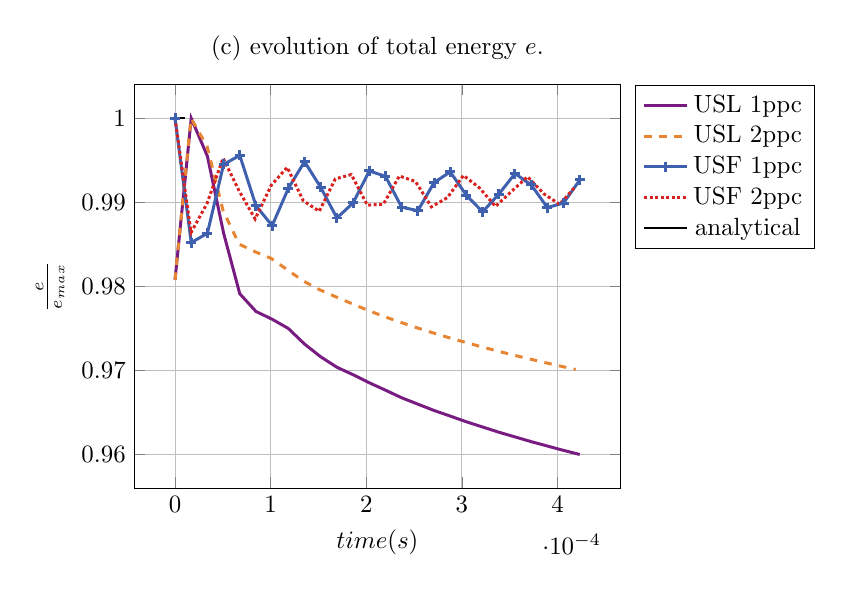
\begin{tikzpicture}[scale=0.9]
\begin{axis}[xlabel=$time (s)$,ylabel=$\frac{e}{e_{max}}$,ymajorgrids=true,xmajorgrids=true,title={(c) evolution of total energy $e$.},legend pos=outer north east]
\addplot[Purple,very thick,mark=none,solid] coordinates {(0.0,0.980776775206) (1.69272151355e-05,1.0) (3.38544302711e-05,0.995486386818) (5.07816454066e-05,0.986335480918) (6.77088605422e-05,0.979118179787) (8.46360756777e-05,0.977011836735) (0.000101563290813,0.976083552705) (0.000118490505949,0.974985958077) (0.000135417721084,0.973132007483) (0.00015234493622,0.971614043952) (0.000169272151355,0.970370597838) (0.000186199366491,0.969484052645) (0.000203126581626,0.968527091175) (0.000220053796762,0.967645365047) (0.000236981011898,0.966743210911) (0.000253908227033,0.965982183586) (0.000270835442169,0.965231974397) (0.000287762657304,0.964563191524) (0.00030468987244,0.96388114719) (0.000321617087575,0.963263530823) (0.000338544302711,0.962646353557) (0.000355471517846,0.962084695394) (0.000372398732982,0.961521764293) (0.000389325948117,0.961001071279) (0.000406253163253,0.960479919884) (0.000423180378389,0.959994795728) };
\addplot[Orange,very thick,mark=none,dashed] coordinates {(0.0,0.980776775206) (1.67562331645e-05,1.0) (3.3512466329e-05,0.996663809337) (5.02686994934e-05,0.98900666995) (6.70249326579e-05,0.985020324447) (8.37811658224e-05,0.984110580813) (0.000100537398987,0.983326915208) (0.000117293632151,0.981979184866) (0.000134049865316,0.980638155666) (0.00015080609848,0.979617302856) (0.000167562331645,0.978778886884) (0.000184318564809,0.977968446843) (0.000201074797974,0.977176694993) (0.000217831031138,0.976440965591) (0.000234587264303,0.975764557777) (0.000251343497467,0.975128766754) (0.000268099730632,0.974522184343) (0.000284855963796,0.973943735564) (0.000301612196961,0.973393220953) (0.000318368430125,0.972867749193) (0.00033512466329,0.972363947434) (0.000351880896454,0.971879647077) (0.000368637129618,0.971413467384) (0.000385393362783,0.970964070517) (0.000402149595947,0.97053007437) (0.000418905829112,0.970110254428) };
\addplot[Blue,very thick,mark=+,solid] coordinates {(0.0,1.0) (1.69272151355e-05,0.985202) (3.38544302711e-05,0.986310925125) (5.07816454066e-05,0.994507638064) (6.77088605422e-05,0.995579868604) (8.46360756777e-05,0.989584575004) (0.000101563290813,0.987225270569) (0.000118490505949,0.991657283729) (0.000135417721084,0.994836102021) (0.00015234493622,0.991773304725) (0.000169272151355,0.988131314159) (0.000186199366491,0.989928559949) (0.000203126581626,0.993725892454) (0.000220053796762,0.993092827557) (0.000236981011898,0.989412077079) (0.000253908227033,0.989007930164) (0.000270835442169,0.992337891088) (0.000287762657304,0.993619763816) (0.00030468987244,0.990831091012) (0.000321617087575,0.988860712515) (0.000338544302711,0.990967493415) (0.000355471517846,0.993415506334) (0.000372398732982,0.99207684926) (0.000389325948117,0.989372657972) (0.000406253163253,0.98991313843) (0.000423180378389,0.992654041387) };
\addplot[Red,very thick,mark=none,densely dotted] coordinates {(0.0,1.0) (1.67562331645e-05,0.9864025) (3.3512466329e-05,0.989873766211) (5.02686994934e-05,0.995255572924) (6.70249326579e-05,0.991355462516) (8.37811658224e-05,0.988011538229) (0.000100537398987,0.992011167376) (0.000117293632151,0.994160481387) (0.000134049865316,0.990189454195) (0.00015080609848,0.988933325063) (0.000167562331645,0.992779930372) (0.000184318564809,0.993300645038) (0.000201074797974,0.989660626012) (0.000217831031138,0.98976821642) (0.000234587264303,0.993129965182) (0.000251343497467,0.992481697852) (0.000268099730632,0.989459518699) (0.000284855963796,0.990567889043) (0.000301612196961,0.993200218105) (0.000318368430125,0.991710475421) (0.00033512466329,0.989506548964) (0.000351880896454,0.99129883371) (0.000368637129618,0.993048080156) (0.000385393362783,0.99103246412) (0.000402149595947,0.989751621209) (0.000418905829112,0.99191164529) };
\addplot[black,thick] coordinates {(0.,1.) (0.00001,1.)};
\legend{USL 1ppc,USL 2ppc,USF 1ppc,USF 2ppc,analytical}
\end{axis}
\end{tikzpicture}
 \phantomsubcaption \label{subfig:US_energies}}
  \caption{MPM solutions of the bars impact problem for various discretizations. (a)--(b) comparison of stress computed with USF and USL formulations and exact solutions (c) numerical total energy evolution. Parameters: $CFL=0.7$ ; $v_0=\frac{1}{200}\sqrt{\frac{E}{\rho}}$.}
  \label{fig:US_diffusion}
\end{figure}
Both ends of the bar are traction free so that this problem is equivalent to an impact of two elastic bars moving toward each other. The bar is discretized by using the MPM in a computational grid composed of $50$ regular cells, each containing either one or two material points (1ppc or 2ppc). Single material points are centered in cells while "cellmate" particles are placed symmetrically with respect to elements centers and are regularly spaced. The exact solution of this problem (see section \ref{subsec:charac_Linear_problems}) consists of two elastic discontinuities emanating from the middle of the bar and propagating leftward and rightward. In figure \ref{fig:US_diffusion}, numerical results provided by the USL and USF implementations of the MPM are compared to the exact solution before reflection of the waves on the boundaries. 

Figures \ref{fig:US_diffusion}\subref{subfig:US_diffusion_10} and \ref{fig:US_diffusion}\subref{subfig:US_diffusion_25} show that both USL and USF solutions oscillate once the elastic front passed. Those oscillations are much more significant in the USF solutions regardless of the number of particles used. Indeed, the noise in USL results quickly reduces so that the correct stress level is reached in the middle region of the bar. Moreover, even though the $1ppc$ and $2ppc$ discretizations provide different results (slightly different for USL), neither of them enables the removal of oscillations. Figure \ref{fig:US_diffusion}\subref{subfig:US_energies} shows, on the other hand, the evolution of numerical total energies resulting from an MPM approximation of kinetic and strain energies:
\begin{align}
  & e^{kin}=\frac{1}{2}\int_\Omega \rho \vect{v}\cdot\vect{v} \:d\Omega \approx \frac{1}{2}\sum_{p=1}^{N_p} m_p \vect{v}^p\cdot\vect{v}^p\\
& e^{strain}= \frac{1}{2}\int_\Omega \rho \tens{\bar{\sigma}}: \nablav \vect{v} \:d\Omega \approx \frac{1}{2}\sum_{p=1}^{N_p} m_p \tens{\bar{\sigma}}^p: \nablav \vect{v}^p
\end{align}
One can see that the USL formulation is more diffusive than the USF for this problem. These results differ from observations made in \cite{Bardenhagen_USF_USL} in which no significant differences for problems involving smooth solutions is noticed. At last, figure \ref{fig:US_velocities} shows the numerical velocities at several time steps. The same observations than before are made by looking at figures \ref{fig:US_velocities}\subref{subfig:US_velo_10} and \ref{fig:US_velocities}\subref{subfig:US_velo_25}, namely numerical oscillations in both USL and USF solutions with bigger peaks in USF one. Nevertheless, a notable numerical artifact that prevents the proper assessment of the velocity occurs at the middle of the bar when two particles per cell are used. This can be partially explained by the oscillating stress field that introduce noise in internal forces as well. However, the velocity field given by USL computation "locks" in the central region although the stress field converges in time to the exact solution (figures \ref{fig:US_diffusion}\subref{subfig:US_diffusion_10} and \ref{fig:US_diffusion}\subref{subfig:US_diffusion_25}), which implies that this issue is not due to the computation of internal forces, but most likely to the convective phase.
\begin{figure}[ht]
  \centering
  {\definecolor{Purple}{RGB}{120,28,129}
\definecolor{Orange}{RGB}{231,133,50}
\definecolor{Blue}{RGB}{63,96,174}
\definecolor{Red}{RGB}{217,33,32}
\definecolor{Duck}{RGB}{83,158,182}
\definecolor{Green}{RGB}{109,179,136}
\definecolor{Yellow}{RGB}{202,184,67}
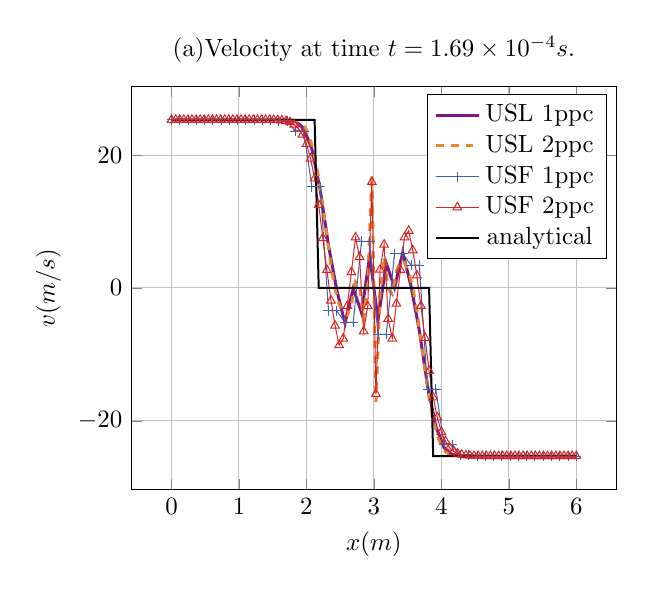
\begin{tikzpicture}[scale=0.9]
\begin{axis}[xlabel=$x (m)$,ylabel=$v (m/s)$,ymajorgrids=true,xmajorgrids=true,title={(a)Velocity at time $t=1.69\times 10^{-4}s.$}]
\addplot[Purple,very thick,mark=none,solid] coordinates {(0.0,25.3184841771) (0.122448979592,25.3184841771) (0.244897959184,25.3184841771) (0.367346938776,25.3184841771) (0.489795918367,25.3184841771) (0.612244897959,25.3184841771) (0.734693877551,25.3184841771) (0.857142857143,25.3184841771) (0.979591836735,25.3184841771) (1.10204081633,25.3184841771) (1.22448979592,25.3184841771) (1.34693877551,25.3184841771) (1.4693877551,25.3184841771) (1.59183673469,25.3184841771) (1.71428571429,25.3184841771) (1.83673469388,25.1149797615) (1.95918367347,24.0545424864) (2.08163265306,20.8743509476) (2.20408163265,14.7547033581) (2.32653061224,6.41598558277) (2.44897959184,-0.244456370035) (2.57142857143,-5.35821612759) (2.69387755102,-0.0619763112976) (2.81632653061,-3.709401685) (2.9387755102,4.8348853161) (3.0612244898,-4.8348853161) (3.18367346939,3.709401685) (3.30612244898,0.0619763112976) (3.42857142857,5.35821612759) (3.55102040816,0.244456370035) (3.67346938776,-6.41598558277) (3.79591836735,-14.7547033581) (3.91836734694,-20.8743509476) (4.04081632653,-24.0545424864) (4.16326530612,-25.1149797615) (4.28571428571,-25.3184841771) (4.40816326531,-25.3184841771) (4.5306122449,-25.3184841771) (4.65306122449,-25.3184841771) (4.77551020408,-25.3184841771) (4.89795918367,-25.3184841771) (5.02040816327,-25.3184841771) (5.14285714286,-25.3184841771) (5.26530612245,-25.3184841771) (5.38775510204,-25.3184841771) (5.51020408163,-25.3184841771) (5.63265306122,-25.3184841771) (5.75510204082,-25.3184841771) (5.87755102041,-25.3184841771) (6.0,-25.3184841771) };
\addplot[Orange,very thick,mark=none,dashed] coordinates {(0.0,25.3184841771) (0.0606060606061,25.3184841771) (0.121212121212,25.3184841771) (0.181818181818,25.3184841771) (0.242424242424,25.3184841771) (0.30303030303,25.3184841771) (0.363636363636,25.3184841771) (0.424242424242,25.3184841771) (0.484848484848,25.3184841771) (0.545454545455,25.3184841771) (0.606060606061,25.3184841771) (0.666666666667,25.3184841771) (0.727272727273,25.3184841771) (0.787878787879,25.3184841771) (0.848484848485,25.3184841771) (0.909090909091,25.3184841771) (0.969696969697,25.3184841771) (1.0303030303,25.3184841771) (1.09090909091,25.3184841771) (1.15151515152,25.3184841771) (1.21212121212,25.3184841771) (1.27272727273,25.3184841771) (1.33333333333,25.3184841771) (1.39393939394,25.3184841771) (1.45454545455,25.3184841771) (1.51515151515,25.3184841771) (1.57575757576,25.3184841771) (1.63636363636,25.3184841771) (1.69696969697,25.3184841771) (1.75757575758,25.3184841771) (1.81818181818,25.251933876) (1.87878787879,25.1188332739) (1.93939393939,24.6493504882) (2.0,23.8434855187) (2.06060606061,22.247450502) (2.12121212121,19.8612454379) (2.18181818182,16.5614104839) (2.24242424242,12.3479456399) (2.30303030303,7.94379399222) (2.36363636364,3.34895554082) (2.42424242424,-0.133198996542) (2.48484848485,-2.50266961986) (2.54545454545,-3.82041358095) (2.60606060606,-4.08643087983) (2.66666666667,-2.50894819569) (2.72727272727,0.91203447147) (2.78787878788,0.178185932665) (2.84848484848,-4.71049381211) (2.90909090909,0.963495780905) (2.9696969697,17.2001547117) (3.0303030303,-17.2001547117) (3.09090909091,-0.963495780905) (3.15151515152,4.7104938121) (3.21212121212,-0.178185932665) (3.27272727273,-0.91203447147) (3.33333333333,2.50894819569) (3.39393939394,4.08643087983) (3.45454545455,3.82041358095) (3.51515151515,2.50266961986) (3.57575757576,0.133198996542) (3.63636363636,-3.34895554082) (3.69696969697,-7.94379399222) (3.75757575758,-12.3479456399) (3.81818181818,-16.5614104839) (3.87878787879,-19.8612454379) (3.93939393939,-22.247450502) (4.0,-23.8434855187) (4.06060606061,-24.6493504882) (4.12121212121,-25.1188332739) (4.18181818182,-25.251933876) (4.24242424242,-25.3184841771) (4.30303030303,-25.3184841771) (4.36363636364,-25.3184841771) (4.42424242424,-25.3184841771) (4.48484848485,-25.3184841771) (4.54545454545,-25.3184841771) (4.60606060606,-25.3184841771) (4.66666666667,-25.3184841771) (4.72727272727,-25.3184841771) (4.78787878788,-25.3184841771) (4.84848484848,-25.3184841771) (4.90909090909,-25.3184841771) (4.9696969697,-25.3184841771) (5.0303030303,-25.3184841771) (5.09090909091,-25.3184841771) (5.15151515152,-25.3184841771) (5.21212121212,-25.3184841771) (5.27272727273,-25.3184841771) (5.33333333333,-25.3184841771) (5.39393939394,-25.3184841771) (5.45454545455,-25.3184841771) (5.51515151515,-25.3184841771) (5.57575757576,-25.3184841771) (5.63636363636,-25.3184841771) (5.69696969697,-25.3184841771) (5.75757575758,-25.3184841771) (5.81818181818,-25.3184841771) (5.87878787879,-25.3184841771) (5.93939393939,-25.3184841771) (6.0,-25.3184841771) };
\addplot[Blue,thin,mark=+,solid] coordinates {(0.0,25.3184841771) (0.122448979592,25.3184841771) (0.244897959184,25.3184841771) (0.367346938776,25.3184841771) (0.489795918367,25.3184841771) (0.612244897959,25.3184841386) (0.734693877551,25.3184841386) (0.857142857143,25.3184789327) (0.979591836735,25.3184789327) (1.10204081633,25.3181863193) (1.22448979592,25.3181863193) (1.34693877551,25.3093479957) (1.4693877551,25.3093479957) (1.59183673469,25.1550198372) (1.71428571429,25.1550198372) (1.83673469388,23.6026380028) (1.95918367347,23.6026380028) (2.08163265306,15.2761405323) (2.20408163265,15.2761405323) (2.32653061224,-3.42382560915) (2.44897959184,-3.42382560915) (2.57142857143,-5.17320665774) (2.69387755102,-5.17320665774) (2.81632653061,6.99898825925) (2.9387755102,6.99898825925) (3.0612244898,-6.99898825925) (3.18367346939,-6.99898825925) (3.30612244898,5.17320665774) (3.42857142857,5.17320665774) (3.55102040816,3.42382560915) (3.67346938776,3.42382560915) (3.79591836735,-15.2761405323) (3.91836734694,-15.2761405323) (4.04081632653,-23.6026380028) (4.16326530612,-23.6026380028) (4.28571428571,-25.1550198372) (4.40816326531,-25.1550198372) (4.5306122449,-25.3093479957) (4.65306122449,-25.3093479957) (4.77551020408,-25.3181863193) (4.89795918367,-25.3181863193) (5.02040816327,-25.3184789327) (5.14285714286,-25.3184789327) (5.26530612245,-25.3184841386) (5.38775510204,-25.3184841386) (5.51020408163,-25.3184841771) (5.63265306122,-25.3184841771) (5.75510204082,-25.3184841771) (5.87755102041,-25.3184841771) (6.0,-25.3184841771) };
\addplot[Red,thin,mark=triangle,solid] coordinates {(0.0,25.3184841771) (0.0606060606061,25.3184841771) (0.121212121212,25.3184841771) (0.181818181818,25.3184841771) (0.242424242424,25.3184841771) (0.30303030303,25.3184841771) (0.363636363636,25.3184841771) (0.424242424242,25.3184841771) (0.484848484848,25.3184841771) (0.545454545455,25.3184841771) (0.606060606061,25.3184841756) (0.666666666667,25.3184841728) (0.727272727273,25.3184841554) (0.787878787879,25.3184841236) (0.848484848485,25.3184837955) (0.909090909091,25.3184831711) (0.969696969697,25.3184803575) (1.0303030303,25.3184753545) (1.09090909091,25.3184471873) (1.15151515152,25.3183958557) (1.21212121212,25.3182145032) (1.27272727273,25.3179031296) (1.33333333333,25.3166920979) (1.39393939394,25.3145814079) (1.45454545455,25.3086270817) (1.51515151515,25.2988291195) (1.57575757576,25.2705514254) (1.63636363636,25.2237939997) (1.69696969697,25.1183204342) (1.75757575758,24.9541307292) (1.81818181818,24.5979538878) (1.87878787879,24.0497899101) (1.93939393939,23.076688448) (2.0,21.6786495014) (2.06060606061,19.4833431738) (2.12121212121,16.4907694654) (2.18181818182,12.4989085572) (2.24242424242,7.50776044936) (2.30303030303,2.70872378788) (2.36363636364,-1.89820142723) (2.42424242424,-5.67144294529) (2.48484848485,-8.61100076632) (2.54545454545,-7.62326403856) (2.60606060606,-2.70823276202) (2.66666666667,2.3712989244) (2.72727272727,7.61533102071) (2.78787878788,4.6503105848) (2.84848484848,-6.52376238331) (2.90909090909,-2.75347810625) (2.9696969697,15.961163416) (3.0303030303,-15.961163416) (3.09090909091,2.75347810625) (3.15151515152,6.52376238331) (3.21212121212,-4.6503105848) (3.27272727273,-7.61533102071) (3.33333333333,-2.3712989244) (3.39393939394,2.70823276202) (3.45454545455,7.62326403856) (3.51515151515,8.61100076632) (3.57575757576,5.67144294529) (3.63636363636,1.89820142723) (3.69696969697,-2.70872378788) (3.75757575758,-7.50776044936) (3.81818181818,-12.4989085572) (3.87878787879,-16.4907694654) (3.93939393939,-19.4833431738) (4.0,-21.6786495014) (4.06060606061,-23.076688448) (4.12121212121,-24.0497899101) (4.18181818182,-24.5979538878) (4.24242424242,-24.9541307292) (4.30303030303,-25.1183204342) (4.36363636364,-25.2237939997) (4.42424242424,-25.2705514254) (4.48484848485,-25.2988291195) (4.54545454545,-25.3086270817) (4.60606060606,-25.3145814079) (4.66666666667,-25.3166920979) (4.72727272727,-25.3179031296) (4.78787878788,-25.3182145032) (4.84848484848,-25.3183958557) (4.90909090909,-25.3184471873) (4.9696969697,-25.3184753545) (5.0303030303,-25.3184803575) (5.09090909091,-25.3184831711) (5.15151515152,-25.3184837955) (5.21212121212,-25.3184841236) (5.27272727273,-25.3184841554) (5.33333333333,-25.3184841728) (5.39393939394,-25.3184841756) (5.45454545455,-25.3184841771) (5.51515151515,-25.3184841771) (5.57575757576,-25.3184841771) (5.63636363636,-25.3184841771) (5.69696969697,-25.3184841771) (5.75757575758,-25.3184841771) (5.81818181818,-25.3184841771) (5.87878787879,-25.3184841771) (5.93939393939,-25.3184841771) (6.0,-25.3184841771) };
\addplot[black,thick,mark=none,solid] coordinates {(0.0,25.3184841771) (0.0606060606061,25.3184841771) (0.121212121212,25.3184841771) (0.181818181818,25.3184841771) (0.242424242424,25.3184841771) (0.30303030303,25.3184841771) (0.363636363636,25.3184841771) (0.424242424242,25.3184841771) (0.484848484848,25.3184841771) (0.545454545455,25.3184841771) (0.606060606061,25.3184841771) (0.666666666667,25.3184841771) (0.727272727273,25.3184841771) (0.787878787879,25.3184841771) (0.848484848485,25.3184841771) (0.909090909091,25.3184841771) (0.969696969697,25.3184841771) (1.0303030303,25.3184841771) (1.09090909091,25.3184841771) (1.15151515152,25.3184841771) (1.21212121212,25.3184841771) (1.27272727273,25.3184841771) (1.33333333333,25.3184841771) (1.39393939394,25.3184841771) (1.45454545455,25.3184841771) (1.51515151515,25.3184841771) (1.57575757576,25.3184841771) (1.63636363636,25.3184841771) (1.69696969697,25.3184841771) (1.75757575758,25.3184841771) (1.81818181818,25.3184841771) (1.87878787879,25.3184841771) (1.93939393939,25.3184841771) (2.0,25.3184841771) (2.06060606061,25.3184841771) (2.12121212121,25.3184841771) (2.18181818182,0.0) (2.24242424242,0.0) (2.30303030303,0.0) (2.36363636364,0.0) (2.42424242424,0.0) (2.48484848485,0.0) (2.54545454545,0.0) (2.60606060606,0.0) (2.66666666667,0.0) (2.72727272727,0.0) (2.78787878788,0.0) (2.84848484848,0.0) (2.90909090909,0.0) (2.9696969697,0.0) (3.0303030303,-0.0) (3.09090909091,-0.0) (3.15151515152,-0.0) (3.21212121212,-0.0) (3.27272727273,-0.0) (3.33333333333,-0.0) (3.39393939394,-0.0) (3.45454545455,-0.0) (3.51515151515,-0.0) (3.57575757576,-0.0) (3.63636363636,-0.0) (3.69696969697,-0.0) (3.75757575758,-0.0) (3.81818181818,-0.0) (3.87878787879,-25.3184841771) (3.93939393939,-25.3184841771) (4.0,-25.3184841771) (4.06060606061,-25.3184841771) (4.12121212121,-25.3184841771) (4.18181818182,-25.3184841771) (4.24242424242,-25.3184841771) (4.30303030303,-25.3184841771) (4.36363636364,-25.3184841771) (4.42424242424,-25.3184841771) (4.48484848485,-25.3184841771) (4.54545454545,-25.3184841771) (4.60606060606,-25.3184841771) (4.66666666667,-25.3184841771) (4.72727272727,-25.3184841771) (4.78787878788,-25.3184841771) (4.84848484848,-25.3184841771) (4.90909090909,-25.3184841771) (4.9696969697,-25.3184841771) (5.0303030303,-25.3184841771) (5.09090909091,-25.3184841771) (5.15151515152,-25.3184841771) (5.21212121212,-25.3184841771) (5.27272727273,-25.3184841771) (5.33333333333,-25.3184841771) (5.39393939394,-25.3184841771) (5.45454545455,-25.3184841771) (5.51515151515,-25.3184841771) (5.57575757576,-25.3184841771) (5.63636363636,-25.3184841771) (5.69696969697,-25.3184841771) (5.75757575758,-25.3184841771) (5.81818181818,-25.3184841771) (5.87878787879,-25.3184841771) (5.93939393939,-25.3184841771) (6.0,-25.3184841771) };
\legend{USL 1ppc,USL 2ppc,USF 1ppc,USF 2ppc,analytical}
\end{axis}
\end{tikzpicture}

%%% Local Variables: 
%%% mode: latex
%%% TeX-master: "../../mainManuscript"
%%% End:
\phantomsubcaption \label{subfig:US_velo_10}}
  {\definecolor{Purple}{RGB}{120,28,129}
\definecolor{Orange}{RGB}{231,133,50}
\definecolor{Blue}{RGB}{63,96,174}
\definecolor{Red}{RGB}{217,33,32}
\definecolor{Duck}{RGB}{83,158,182}
\definecolor{Green}{RGB}{109,179,136}
\definecolor{Yellow}{RGB}{202,184,67}
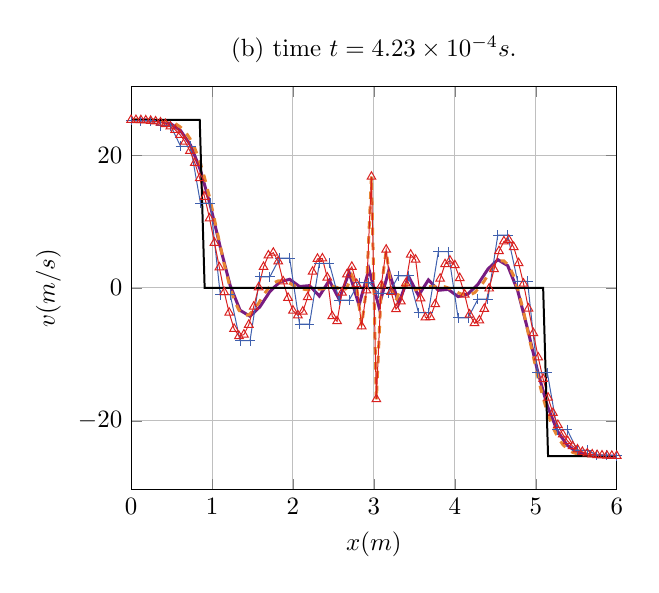
\begin{tikzpicture}[scale=0.9]
\begin{axis}[xlabel=$x (m)$,ylabel=$v (m/s)$,ymajorgrids=true,xmajorgrids=true,title={(b) time $t=4.23 \times 10^{-4}s$.},xmin=0.,xmax=6.]
\addplot[Purple,very thick,mark=none,solid] coordinates {(0.0,25.3179577559) (0.122448979592,25.3125244526) (0.244897959184,25.2804932478) (0.367346938776,25.1489907367) (0.489795918367,24.7341796044) (0.612244897959,23.6864809647) (0.734693877551,21.5118739395) (0.857142857143,17.7671095652) (0.979591836735,12.4121755247) (1.10204081633,6.14683940753) (1.22448979592,0.373716046882) (1.34693877551,-3.3616057723) (1.4693877551,-4.26176674269) (1.59183673469,-2.83406587609) (1.71428571429,-0.55562049587) (1.83673469388,0.901404345798) (1.95918367347,1.30403292578) (2.08163265306,0.214501074535) (2.20408163265,0.352209313776) (2.32653061224,-1.21718822558) (2.44897959184,1.14054029809) (2.57142857143,-1.72149525556) (2.69387755102,2.335373076) (2.81632653061,-2.59610029814) (2.9387755102,2.82071480229) (3.0612244898,-2.82071480229) (3.18367346939,2.59610029814) (3.30612244898,-2.335373076) (3.42857142857,1.72149525556) (3.55102040816,-1.14054029809) (3.67346938776,1.21718822558) (3.79591836735,-0.352209313776) (3.91836734694,-0.214501074535) (4.04081632653,-1.30403292578) (4.16326530612,-0.901404345798) (4.28571428571,0.55562049587) (4.40816326531,2.83406587609) (4.5306122449,4.26176674269) (4.65306122449,3.3616057723) (4.77551020408,-0.373716046882) (4.89795918367,-6.14683940753) (5.02040816327,-12.4121755247) (5.14285714286,-17.7671095652) (5.26530612245,-21.5118739395) (5.38775510204,-23.6864809647) (5.51020408163,-24.7341796044) (5.63265306122,-25.1489907367) (5.75510204082,-25.2804932478) (5.87755102041,-25.3125244526) (6.0,-25.3179577559) };
\addplot[Orange,very thick,mark=none,dashed] coordinates {(0.0,25.3184113784) (0.0606060606061,25.3182657812) (0.121212121212,25.3171343813) (0.181818181818,25.3150171787) (0.242424242424,25.3062460446) (0.30303030303,25.2908209787) (0.363636363636,25.2461773758) (0.424242424242,25.1723152357) (0.484848484848,25.0062868064) (0.545454545455,24.748092088) (0.606060606061,24.2720385643) (0.666666666667,23.5781262352) (0.727272727273,22.4951335769) (0.787878787879,21.0230605893) (0.848484848485,19.0428242456) (0.909090909091,16.5544245458) (0.969696969697,13.6460768618) (1.0303030303,10.3177811934) (1.09090909091,6.94923058708) (1.15151515152,3.54042504293) (1.21212121212,0.626561316633) (1.27272727273,-1.79236059183) (1.33333333333,-3.36301978655) (1.39393939394,-4.08541626753) (1.45454545455,-4.06554257142) (1.51515151515,-3.30339869822) (1.57575757576,-2.29577774705) (1.63636363636,-1.04267971791) (1.69696969697,-0.0393881478233) (1.75757575758,0.714096963215) (1.81818181818,1.07591385411) (1.87878787879,1.04606252486) (1.93939393939,0.832069940855) (2.0,0.433936102092) (2.06060606061,0.100491892604) (2.12121212121,-0.168262687611) (2.18181818182,-0.281962807299) (2.24242424242,-0.24060846646) (2.30303030303,-0.19473430746) (2.36363636364,-0.144340330301) (2.42424242424,0.0103021847971) (2.48484848485,0.269193237834) (2.54545454545,0.0743373654573) (2.60606060606,-0.574265432333) (2.66666666667,0.0252212025898) (2.72727272727,1.87279727022) (2.78787878788,-0.017779131944) (2.84848484848,-5.64650800392) (2.90909090909,-0.0160332856532) (2.9696969697,16.8736450228) (3.0303030303,-16.8736450228) (3.09090909091,0.0160332856532) (3.15151515152,5.64650800392) (3.21212121212,0.017779131944) (3.27272727273,-1.87279727022) (3.33333333333,-0.0252212025898) (3.39393939394,0.574265432333) (3.45454545455,-0.0743373654573) (3.51515151515,-0.269193237834) (3.57575757576,-0.0103021847971) (3.63636363636,0.144340330301) (3.69696969697,0.19473430746) (3.75757575758,0.24060846646) (3.81818181818,0.281962807299) (3.87878787879,0.168262687611) (3.93939393939,-0.100491892604) (4.0,-0.433936102092) (4.06060606061,-0.832069940855) (4.12121212121,-1.04606252486) (4.18181818182,-1.07591385411) (4.24242424242,-0.714096963215) (4.30303030303,0.0393881478233) (4.36363636364,1.04267971791) (4.42424242424,2.29577774705) (4.48484848485,3.30339869822) (4.54545454545,4.06554257142) (4.60606060606,4.08541626753) (4.66666666667,3.36301978655) (4.72727272727,1.79236059183) (4.78787878788,-0.626561316633) (4.84848484848,-3.54042504293) (4.90909090909,-6.94923058708) (4.9696969697,-10.3177811934) (5.0303030303,-13.6460768618) (5.09090909091,-16.5544245458) (5.15151515152,-19.0428242456) (5.21212121212,-21.0230605893) (5.27272727273,-22.4951335769) (5.33333333333,-23.5781262352) (5.39393939394,-24.2720385643) (5.45454545455,-24.748092088) (5.51515151515,-25.0062868064) (5.57575757576,-25.1723152357) (5.63636363636,-25.2461773758) (5.69696969697,-25.2908209787) (5.75757575758,-25.3062460446) (5.81818181818,-25.3150171787) (5.87878787879,-25.3171343813) (5.93939393939,-25.3182657812) (6.0,-25.3184113784) };
\addplot[Blue,thin,mark=+,solid] coordinates {(0.0,25.278692227) (0.122448979592,25.1632638972) (0.244897959184,25.1632638972) (0.367346938776,24.4134945697) (0.489795918367,24.4134945697) (0.612244897959,21.3339382893) (0.734693877551,21.3339382893) (0.857142857143,12.7864947989) (0.979591836735,12.7864947989) (1.10204081633,-1.00143026403) (1.22448979592,-1.00143026403) (1.34693877551,-7.94234859658) (1.4693877551,-7.94234859658) (1.59183673469,1.666718506) (1.71428571429,1.666718506) (1.83673469388,4.4983018773) (1.95918367347,4.4983018773) (2.08163265306,-5.4528024961) (2.20408163265,-5.4528024961) (2.32653061224,3.70951010765) (2.44897959184,3.70951010765) (2.57142857143,-1.8372342386) (2.69387755102,-1.8372342386) (2.81632653061,0.817767529336) (2.9387755102,0.817767529337) (3.0612244898,-0.817767529337) (3.18367346939,-0.817767529336) (3.30612244898,1.8372342386) (3.42857142857,1.8372342386) (3.55102040816,-3.70951010765) (3.67346938776,-3.70951010765) (3.79591836735,5.4528024961) (3.91836734694,5.4528024961) (4.04081632653,-4.4983018773) (4.16326530612,-4.4983018773) (4.28571428571,-1.666718506) (4.40816326531,-1.666718506) (4.5306122449,7.94234859658) (4.65306122449,7.94234859658) (4.77551020408,1.00143026403) (4.89795918367,1.00143026403) (5.02040816327,-12.7864947989) (5.14285714286,-12.7864947989) (5.26530612245,-21.3339382893) (5.38775510204,-21.3339382893) (5.51020408163,-24.4134945697) (5.63265306122,-24.4134945697) (5.75510204082,-25.1632638972) (5.87755102041,-25.1632638972) (6.0,-25.278692227) };
\addplot[Red,thin,mark=triangle,solid] coordinates {(0.0,25.2925663718) (0.0606060606061,25.2843839677) (0.121212121212,25.2634771526) (0.181818181818,25.2298459266) (0.242424242424,25.166861976) (0.30303030303,25.074525301) (0.363636363636,24.9151607465) (0.424242424242,24.6887683126) (0.484848484848,24.3234854983) (0.545454545455,23.8193123035) (0.606060606061,23.0610017936) (0.666666666667,22.0485539687) (0.727272727273,20.638560445) (0.787878787879,18.8310212227) (0.848484848485,16.5222107775) (0.909090909091,13.7121291096) (0.969696969697,10.4726131337) (1.0303030303,6.80366284984) (1.09090909091,3.09745596005) (1.15151515152,-0.646007535703) (1.21212121212,-3.7294710718) (1.27272727273,-6.15293464823) (1.33333333333,-7.25044901317) (1.39393939394,-7.02201416662) (1.45454545455,-5.54409239748) (1.51515151515,-2.81668370575) (1.57575757576,0.0833596298948) (1.63636363636,3.15603760945) (1.69696969697,4.89643176607) (1.75757575758,5.30454209975) (1.81818181818,4.00211543869) (1.87878787879,0.98915178291) (1.93939393939,-1.48619261955) (2.0,-3.42391776869) (2.06060606061,-4.1204907004) (2.12121212121,-3.57591141468) (2.18181818182,-1.3875328666) (2.24242424242,2.44464494385) (2.30303030303,4.38796385565) (2.36363636364,4.44242386881) (2.42424242424,1.55990936166) (2.48484848485,-4.2595796658) (2.54545454545,-5.01317341167) (2.60606060606,-0.700871875953) (2.66666666667,2.03314306079) (2.72727272727,3.18887139857) (2.78787878788,0.588067826574) (2.84848484848,-5.76926765519) (2.90909090909,-0.381330502781) (2.9696969697,16.7518792838) (3.0303030303,-16.7518792838) (3.09090909091,0.381330502781) (3.15151515152,5.76926765519) (3.21212121212,-0.588067826574) (3.27272727273,-3.18887139857) (3.33333333333,-2.03314306079) (3.39393939394,0.700871875953) (3.45454545455,5.01317341167) (3.51515151515,4.2595796658) (3.57575757576,-1.55990936166) (3.63636363636,-4.44242386881) (3.69696969697,-4.38796385565) (3.75757575758,-2.44464494385) (3.81818181818,1.3875328666) (3.87878787879,3.57591141468) (3.93939393939,4.1204907004) (4.0,3.42391776869) (4.06060606061,1.48619261955) (4.12121212121,-0.98915178291) (4.18181818182,-4.00211543869) (4.24242424242,-5.30454209975) (4.30303030303,-4.89643176607) (4.36363636364,-3.15603760945) (4.42424242424,-0.0833596298948) (4.48484848485,2.81668370575) (4.54545454545,5.54409239748) (4.60606060606,7.02201416662) (4.66666666667,7.25044901317) (4.72727272727,6.15293464823) (4.78787878788,3.7294710718) (4.84848484848,0.646007535703) (4.90909090909,-3.09745596005) (4.9696969697,-6.80366284984) (5.0303030303,-10.4726131337) (5.09090909091,-13.7121291096) (5.15151515152,-16.5222107775) (5.21212121212,-18.8310212227) (5.27272727273,-20.638560445) (5.33333333333,-22.0485539687) (5.39393939394,-23.0610017936) (5.45454545455,-23.8193123035) (5.51515151515,-24.3234854983) (5.57575757576,-24.6887683126) (5.63636363636,-24.9151607465) (5.69696969697,-25.074525301) (5.75757575758,-25.166861976) (5.81818181818,-25.2298459266) (5.87878787879,-25.2634771526) (5.93939393939,-25.2843839677) (6.0,-25.2925663718) };
\addplot[black,thick,mark=none,solid] coordinates {(0.0,25.3184841771) (0.0606060606061,25.3184841771) (0.121212121212,25.3184841771) (0.181818181818,25.3184841771) (0.242424242424,25.3184841771) (0.30303030303,25.3184841771) (0.363636363636,25.3184841771) (0.424242424242,25.3184841771) (0.484848484848,25.3184841771) (0.545454545455,25.3184841771) (0.606060606061,25.3184841771) (0.666666666667,25.3184841771) (0.727272727273,25.3184841771) (0.787878787879,25.3184841771) (0.848484848485,25.3184841771) (0.909090909091,0.0) (0.969696969697,0.0) (1.0303030303,0.0) (1.09090909091,0.0) (1.15151515152,0.0) (1.21212121212,0.0) (1.27272727273,0.0) (1.33333333333,0.0) (1.39393939394,0.0) (1.45454545455,0.0) (1.51515151515,0.0) (1.57575757576,0.0) (1.63636363636,0.0) (1.69696969697,0.0) (1.75757575758,0.0) (1.81818181818,0.0) (1.87878787879,0.0) (1.93939393939,0.0) (2.0,0.0) (2.06060606061,0.0) (2.12121212121,0.0) (2.18181818182,0.0) (2.24242424242,0.0) (2.30303030303,0.0) (2.36363636364,0.0) (2.42424242424,0.0) (2.48484848485,0.0) (2.54545454545,0.0) (2.60606060606,0.0) (2.66666666667,0.0) (2.72727272727,0.0) (2.78787878788,0.0) (2.84848484848,0.0) (2.90909090909,0.0) (2.9696969697,0.0) (3.0303030303,-0.0) (3.09090909091,-0.0) (3.15151515152,-0.0) (3.21212121212,-0.0) (3.27272727273,-0.0) (3.33333333333,-0.0) (3.39393939394,-0.0) (3.45454545455,-0.0) (3.51515151515,-0.0) (3.57575757576,-0.0) (3.63636363636,-0.0) (3.69696969697,-0.0) (3.75757575758,-0.0) (3.81818181818,-0.0) (3.87878787879,-0.0) (3.93939393939,-0.0) (4.0,-0.0) (4.06060606061,-0.0) (4.12121212121,-0.0) (4.18181818182,-0.0) (4.24242424242,-0.0) (4.30303030303,-0.0) (4.36363636364,-0.0) (4.42424242424,-0.0) (4.48484848485,-0.0) (4.54545454545,-0.0) (4.60606060606,-0.0) (4.66666666667,-0.0) (4.72727272727,-0.0) (4.78787878788,-0.0) (4.84848484848,-0.0) (4.90909090909,-0.0) (4.9696969697,-0.0) (5.0303030303,-0.0) (5.09090909091,-0.0) (5.15151515152,-25.3184841771) (5.21212121212,-25.3184841771) (5.27272727273,-25.3184841771) (5.33333333333,-25.3184841771) (5.39393939394,-25.3184841771) (5.45454545455,-25.3184841771) (5.51515151515,-25.3184841771) (5.57575757576,-25.3184841771) (5.63636363636,-25.3184841771) (5.69696969697,-25.3184841771) (5.75757575758,-25.3184841771) (5.81818181818,-25.3184841771) (5.87878787879,-25.3184841771) (5.93939393939,-25.3184841771) (6.0,-25.3184841771) };
%\legend{USL 1ppc,USL 2ppc,USF 1ppc,USF 2ppc,analytical}
\end{axis}
\end{tikzpicture}
%%% Local Variables:
%%% mode: latex
%%% TeX-master: "../../mainManuscript"
%%% End:
\phantomsubcaption \label{subfig:US_velo_25}}
  \caption{Comparison between exact, USF and USL velocities of the bars impact problem for various discretizations.}
  \label{fig:US_velocities}
\end{figure}

Since the back-mapping is known to be responsible for noise introduced in MPM solution \cite{Mass_Flip}, we propose to project the velocity onto particles by a simple interpolation, as it is done in PIC:
%Since the back-mapping of fields from the grid to material points is known to be responsible for noise introduced in MPM solution , we propose to project fields onto particles as it is done in PIC instead, that is by a simple interpolation:
\begin{equation}
  \label{eq:PIC_Back-mapping}
  \vect{v}^{p,n+1}=\sum_{i=1}^{N_n} S_{ip}\vect{v}^{i,n+1}
\end{equation}
Particles positions are next updated as in FLIP, with the nodal velocity \eqref{eq:position_update}, thus amounting to deform Lagrangian particles with the grid and exactly satisfy the relation $\vect{\dot{x}}^p=\vect{v}^p$, which is not the case in MPM. It is then worth noticing that the weak form \eqref{eq:mpm_discrete_weak} is based on the definition \eqref{eq:PIC_Back-mapping}, this projection seems therefore more consistent.

The comparison between MPM using either PIC or FLIP mapping and exact velocities is plotted in figures \ref{fig:MPM_velocities}\subref{subfig:MPM_velo_10} and \ref{fig:MPM_velocities}\subref{subfig:MPM_velo_25}
\begin{figure}[h!]
  \centering
  {\definecolor{Purple}{RGB}{120,28,129}
\definecolor{Orange}{RGB}{231,133,50}
\definecolor{Blue}{RGB}{63,96,174}
\definecolor{Red}{RGB}{217,33,32}
\definecolor{Duck}{RGB}{83,158,182}
\definecolor{Green}{RGB}{109,179,136}
\definecolor{Yellow}{RGB}{202,184,67}
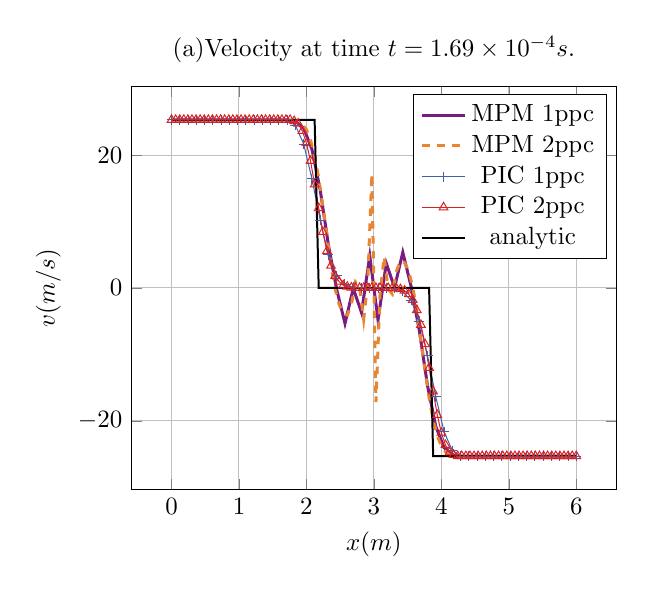
\begin{tikzpicture}[scale=0.9]
\begin{axis}[xlabel=$x (m)$,ylabel=$v (m/s)$,ymajorgrids=true,xmajorgrids=true,title={(a)Velocity at time $t=1.69\times 10^{-4}s.$}]
\addplot[Purple,very thick,mark=none,solid] coordinates {(0.0,25.3184841771) (0.122448979592,25.3184841771) (0.244897959184,25.3184841771) (0.367346938776,25.3184841771) (0.489795918367,25.3184841771) (0.612244897959,25.3184841771) (0.734693877551,25.3184841771) (0.857142857143,25.3184841771) (0.979591836735,25.3184841771) (1.10204081633,25.3184841771) (1.22448979592,25.3184841771) (1.34693877551,25.3184841771) (1.4693877551,25.3184841771) (1.59183673469,25.3184841771) (1.71428571429,25.3184841771) (1.83673469388,25.1149797615) (1.95918367347,24.0545424864) (2.08163265306,20.8743509476) (2.20408163265,14.7547033581) (2.32653061224,6.41598558277) (2.44897959184,-0.244456370035) (2.57142857143,-5.35821612759) (2.69387755102,-0.0619763112976) (2.81632653061,-3.709401685) (2.9387755102,4.8348853161) (3.0612244898,-4.8348853161) (3.18367346939,3.709401685) (3.30612244898,0.0619763112976) (3.42857142857,5.35821612759) (3.55102040816,0.244456370035) (3.67346938776,-6.41598558277) (3.79591836735,-14.7547033581) (3.91836734694,-20.8743509476) (4.04081632653,-24.0545424864) (4.16326530612,-25.1149797615) (4.28571428571,-25.3184841771) (4.40816326531,-25.3184841771) (4.5306122449,-25.3184841771) (4.65306122449,-25.3184841771) (4.77551020408,-25.3184841771) (4.89795918367,-25.3184841771) (5.02040816327,-25.3184841771) (5.14285714286,-25.3184841771) (5.26530612245,-25.3184841771) (5.38775510204,-25.3184841771) (5.51020408163,-25.3184841771) (5.63265306122,-25.3184841771) (5.75510204082,-25.3184841771) (5.87755102041,-25.3184841771) (6.0,-25.3184841771) };
\addplot[Orange,very thick,mark=none,dashed] coordinates {(0.0,25.3184841771) (0.0606060606061,25.3184841771) (0.121212121212,25.3184841771) (0.181818181818,25.3184841771) (0.242424242424,25.3184841771) (0.30303030303,25.3184841771) (0.363636363636,25.3184841771) (0.424242424242,25.3184841771) (0.484848484848,25.3184841771) (0.545454545455,25.3184841771) (0.606060606061,25.3184841771) (0.666666666667,25.3184841771) (0.727272727273,25.3184841771) (0.787878787879,25.3184841771) (0.848484848485,25.3184841771) (0.909090909091,25.3184841771) (0.969696969697,25.3184841771) (1.0303030303,25.3184841771) (1.09090909091,25.3184841771) (1.15151515152,25.3184841771) (1.21212121212,25.3184841771) (1.27272727273,25.3184841771) (1.33333333333,25.3184841771) (1.39393939394,25.3184841771) (1.45454545455,25.3184841771) (1.51515151515,25.3184841771) (1.57575757576,25.3184841771) (1.63636363636,25.3184841771) (1.69696969697,25.3184841771) (1.75757575758,25.3184841771) (1.81818181818,25.251933876) (1.87878787879,25.1188332739) (1.93939393939,24.6493504882) (2.0,23.8434855187) (2.06060606061,22.247450502) (2.12121212121,19.8612454379) (2.18181818182,16.5614104839) (2.24242424242,12.3479456399) (2.30303030303,7.94379399222) (2.36363636364,3.34895554082) (2.42424242424,-0.133198996542) (2.48484848485,-2.50266961986) (2.54545454545,-3.82041358095) (2.60606060606,-4.08643087983) (2.66666666667,-2.50894819569) (2.72727272727,0.91203447147) (2.78787878788,0.178185932665) (2.84848484848,-4.71049381211) (2.90909090909,0.963495780905) (2.9696969697,17.2001547117) (3.0303030303,-17.2001547117) (3.09090909091,-0.963495780905) (3.15151515152,4.7104938121) (3.21212121212,-0.178185932665) (3.27272727273,-0.91203447147) (3.33333333333,2.50894819569) (3.39393939394,4.08643087983) (3.45454545455,3.82041358095) (3.51515151515,2.50266961986) (3.57575757576,0.133198996542) (3.63636363636,-3.34895554082) (3.69696969697,-7.94379399222) (3.75757575758,-12.3479456399) (3.81818181818,-16.5614104839) (3.87878787879,-19.8612454379) (3.93939393939,-22.247450502) (4.0,-23.8434855187) (4.06060606061,-24.6493504882) (4.12121212121,-25.1188332739) (4.18181818182,-25.251933876) (4.24242424242,-25.3184841771) (4.30303030303,-25.3184841771) (4.36363636364,-25.3184841771) (4.42424242424,-25.3184841771) (4.48484848485,-25.3184841771) (4.54545454545,-25.3184841771) (4.60606060606,-25.3184841771) (4.66666666667,-25.3184841771) (4.72727272727,-25.3184841771) (4.78787878788,-25.3184841771) (4.84848484848,-25.3184841771) (4.90909090909,-25.3184841771) (4.9696969697,-25.3184841771) (5.0303030303,-25.3184841771) (5.09090909091,-25.3184841771) (5.15151515152,-25.3184841771) (5.21212121212,-25.3184841771) (5.27272727273,-25.3184841771) (5.33333333333,-25.3184841771) (5.39393939394,-25.3184841771) (5.45454545455,-25.3184841771) (5.51515151515,-25.3184841771) (5.57575757576,-25.3184841771) (5.63636363636,-25.3184841771) (5.69696969697,-25.3184841771) (5.75757575758,-25.3184841771) (5.81818181818,-25.3184841771) (5.87878787879,-25.3184841771) (5.93939393939,-25.3184841771) (6.0,-25.3184841771) };
\addplot[Blue,thin,mark=+,solid] coordinates {(0.0,25.3184841771) (0.122448979592,25.3184841771) (0.244897959184,25.3184841771) (0.367346938776,25.3184841771) (0.489795918367,25.3184841771) (0.612244897959,25.3184841771) (0.734693877551,25.3184841771) (0.857142857143,25.3184841771) (0.979591836735,25.3184841771) (1.10204081633,25.3184841771) (1.22448979592,25.3184841771) (1.34693877551,25.3184841771) (1.4693877551,25.3184841771) (1.59183673469,25.3184841771) (1.71428571429,25.3184841771) (1.83673469388,24.4761330084) (1.95918367347,21.6789610487) (2.08163265306,16.4171127559) (2.20408163265,10.2176854187) (2.32653061224,4.99697293397) (2.44897959184,1.87425322807) (2.57142857143,0.532987126345) (2.69387755102,0.0744368580376) (2.81632653061,0.0446687900239) (2.9387755102,-0.0367040274884) (3.0612244898,0.0367040274884) (3.18367346939,-0.0446687900239) (3.30612244898,-0.0744368580376) (3.42857142857,-0.532987126345) (3.55102040816,-1.87425322807) (3.67346938776,-4.99697293397) (3.79591836735,-10.2176854187) (3.91836734694,-16.4171127559) (4.04081632653,-21.6789610487) (4.16326530612,-24.4761330084) (4.28571428571,-25.3184841771) (4.40816326531,-25.3184841771) (4.5306122449,-25.3184841771) (4.65306122449,-25.3184841771) (4.77551020408,-25.3184841771) (4.89795918367,-25.3184841771) (5.02040816327,-25.3184841771) (5.14285714286,-25.3184841771) (5.26530612245,-25.3184841771) (5.38775510204,-25.3184841771) (5.51020408163,-25.3184841771) (5.63265306122,-25.3184841771) (5.75510204082,-25.3184841771) (5.87755102041,-25.3184841771) (6.0,-25.3184841771) };
\addplot[Red,thin,mark=triangle,solid] coordinates {(0.0,25.3184841771) (0.0606060606061,25.3184841771) (0.121212121212,25.3184841771) (0.181818181818,25.3184841771) (0.242424242424,25.3184841771) (0.30303030303,25.3184841771) (0.363636363636,25.3184841771) (0.424242424242,25.3184841771) (0.484848484848,25.3184841771) (0.545454545455,25.3184841771) (0.606060606061,25.3184841771) (0.666666666667,25.3184841771) (0.727272727273,25.3184841771) (0.787878787879,25.3184841771) (0.848484848485,25.3184841771) (0.909090909091,25.3184841771) (0.969696969697,25.3184841771) (1.0303030303,25.3184841771) (1.09090909091,25.3184841771) (1.15151515152,25.3184841771) (1.21212121212,25.3184841771) (1.27272727273,25.3184841771) (1.33333333333,25.3184841771) (1.39393939394,25.3184841771) (1.45454545455,25.3184841771) (1.51515151515,25.3184841771) (1.57575757576,25.3184841771) (1.63636363636,25.3184841771) (1.69696969697,25.3184841771) (1.75757575758,25.3184841771) (1.81818181818,25.1281304409) (1.87878787879,24.7474229685) (1.93939393939,23.6387415979) (2.0,21.8020863292) (2.06060606061,19.1201129846) (2.12121212121,15.5928215642) (2.18181818182,12.0349431808) (2.24242424242,8.44647783432) (2.30303030303,5.5505820269) (2.36363636364,3.3472557585) (2.42424242424,1.81296030454) (2.48484848485,0.947695665037) (2.54545454545,0.405594826726) (2.60606060606,0.186657789609) (2.66666666667,0.0594742699364) (2.72727272727,0.0240442677077) (2.78787878788,0.00485504304949) (2.84848484848,0.00190659596188) (2.90909090909,0.000324279313551) (2.9696969697,0.000108093104517) (3.0303030303,-0.000108093104518) (3.09090909091,-0.000324279313554) (3.15151515152,-0.00190659596188) (3.21212121212,-0.0048550430495) (3.27272727273,-0.0240442677077) (3.33333333333,-0.0594742699364) (3.39393939394,-0.186657789609) (3.45454545455,-0.405594826726) (3.51515151515,-0.947695665037) (3.57575757576,-1.81296030454) (3.63636363636,-3.3472557585) (3.69696969697,-5.5505820269) (3.75757575758,-8.44647783432) (3.81818181818,-12.0349431808) (3.87878787879,-15.5928215642) (3.93939393939,-19.1201129846) (4.0,-21.8020863292) (4.06060606061,-23.6387415979) (4.12121212121,-24.7474229685) (4.18181818182,-25.1281304409) (4.24242424242,-25.3184841771) (4.30303030303,-25.3184841771) (4.36363636364,-25.3184841771) (4.42424242424,-25.3184841771) (4.48484848485,-25.3184841771) (4.54545454545,-25.3184841771) (4.60606060606,-25.3184841771) (4.66666666667,-25.3184841771) (4.72727272727,-25.3184841771) (4.78787878788,-25.3184841771) (4.84848484848,-25.3184841771) (4.90909090909,-25.3184841771) (4.9696969697,-25.3184841771) (5.0303030303,-25.3184841771) (5.09090909091,-25.3184841771) (5.15151515152,-25.3184841771) (5.21212121212,-25.3184841771) (5.27272727273,-25.3184841771) (5.33333333333,-25.3184841771) (5.39393939394,-25.3184841771) (5.45454545455,-25.3184841771) (5.51515151515,-25.3184841771) (5.57575757576,-25.3184841771) (5.63636363636,-25.3184841771) (5.69696969697,-25.3184841771) (5.75757575758,-25.3184841771) (5.81818181818,-25.3184841771) (5.87878787879,-25.3184841771) (5.93939393939,-25.3184841771) (6.0,-25.3184841771) };
\addplot[black,thick,mark=none,solid] coordinates {(0.0,25.3184841771) (0.0606060606061,25.3184841771) (0.121212121212,25.3184841771) (0.181818181818,25.3184841771) (0.242424242424,25.3184841771) (0.30303030303,25.3184841771) (0.363636363636,25.3184841771) (0.424242424242,25.3184841771) (0.484848484848,25.3184841771) (0.545454545455,25.3184841771) (0.606060606061,25.3184841771) (0.666666666667,25.3184841771) (0.727272727273,25.3184841771) (0.787878787879,25.3184841771) (0.848484848485,25.3184841771) (0.909090909091,25.3184841771) (0.969696969697,25.3184841771) (1.0303030303,25.3184841771) (1.09090909091,25.3184841771) (1.15151515152,25.3184841771) (1.21212121212,25.3184841771) (1.27272727273,25.3184841771) (1.33333333333,25.3184841771) (1.39393939394,25.3184841771) (1.45454545455,25.3184841771) (1.51515151515,25.3184841771) (1.57575757576,25.3184841771) (1.63636363636,25.3184841771) (1.69696969697,25.3184841771) (1.75757575758,25.3184841771) (1.81818181818,25.3184841771) (1.87878787879,25.3184841771) (1.93939393939,25.3184841771) (2.0,25.3184841771) (2.06060606061,25.3184841771) (2.12121212121,25.3184841771) (2.18181818182,0.0) (2.24242424242,0.0) (2.30303030303,0.0) (2.36363636364,0.0) (2.42424242424,0.0) (2.48484848485,0.0) (2.54545454545,0.0) (2.60606060606,0.0) (2.66666666667,0.0) (2.72727272727,0.0) (2.78787878788,0.0) (2.84848484848,0.0) (2.90909090909,0.0) (2.9696969697,0.0) (3.0303030303,-0.0) (3.09090909091,-0.0) (3.15151515152,-0.0) (3.21212121212,-0.0) (3.27272727273,-0.0) (3.33333333333,-0.0) (3.39393939394,-0.0) (3.45454545455,-0.0) (3.51515151515,-0.0) (3.57575757576,-0.0) (3.63636363636,-0.0) (3.69696969697,-0.0) (3.75757575758,-0.0) (3.81818181818,-0.0) (3.87878787879,-25.3184841771) (3.93939393939,-25.3184841771) (4.0,-25.3184841771) (4.06060606061,-25.3184841771) (4.12121212121,-25.3184841771) (4.18181818182,-25.3184841771) (4.24242424242,-25.3184841771) (4.30303030303,-25.3184841771) (4.36363636364,-25.3184841771) (4.42424242424,-25.3184841771) (4.48484848485,-25.3184841771) (4.54545454545,-25.3184841771) (4.60606060606,-25.3184841771) (4.66666666667,-25.3184841771) (4.72727272727,-25.3184841771) (4.78787878788,-25.3184841771) (4.84848484848,-25.3184841771) (4.90909090909,-25.3184841771) (4.9696969697,-25.3184841771) (5.0303030303,-25.3184841771) (5.09090909091,-25.3184841771) (5.15151515152,-25.3184841771) (5.21212121212,-25.3184841771) (5.27272727273,-25.3184841771) (5.33333333333,-25.3184841771) (5.39393939394,-25.3184841771) (5.45454545455,-25.3184841771) (5.51515151515,-25.3184841771) (5.57575757576,-25.3184841771) (5.63636363636,-25.3184841771) (5.69696969697,-25.3184841771) (5.75757575758,-25.3184841771) (5.81818181818,-25.3184841771) (5.87878787879,-25.3184841771) (5.93939393939,-25.3184841771) (6.0,-25.3184841771) };
\legend{MPM 1ppc,MPM 2ppc,PIC 1ppc,PIC 2ppc,analytic}
\end{axis}
\end{tikzpicture}
%%% Local Variables: 
%%% mode: latex
%%% TeX-master: "../../mainManuscript"
%%% End:
\phantomsubcaption \label{subfig:MPM_velo_10}}
  {\definecolor{Purple}{RGB}{120,28,129}
\definecolor{Orange}{RGB}{231,133,50}
\definecolor{Blue}{RGB}{63,96,174}
\definecolor{Red}{RGB}{217,33,32}
\definecolor{Duck}{RGB}{83,158,182}
\definecolor{Green}{RGB}{109,179,136}
\definecolor{Yellow}{RGB}{202,184,67}
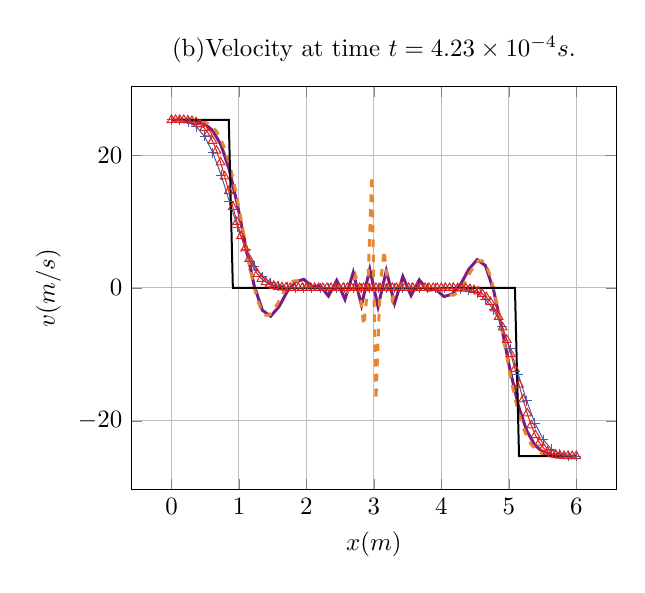
\begin{tikzpicture}[scale=0.9]
\begin{axis}[xlabel=$x (m)$,ylabel=$v (m/s)$,ymajorgrids=true,xmajorgrids=true,title={(b)Velocity at time $t=4.23\times 10^{-4}s.$}]
\addplot[Purple,very thick,mark=none,solid] coordinates {(0.0,25.3179577559) (0.122448979592,25.3125244526) (0.244897959184,25.2804932478) (0.367346938776,25.1489907367) (0.489795918367,24.7341796044) (0.612244897959,23.6864809647) (0.734693877551,21.5118739395) (0.857142857143,17.7671095652) (0.979591836735,12.4121755247) (1.10204081633,6.14683940753) (1.22448979592,0.373716046882) (1.34693877551,-3.3616057723) (1.4693877551,-4.26176674269) (1.59183673469,-2.83406587609) (1.71428571429,-0.55562049587) (1.83673469388,0.901404345798) (1.95918367347,1.30403292578) (2.08163265306,0.214501074535) (2.20408163265,0.352209313776) (2.32653061224,-1.21718822558) (2.44897959184,1.14054029809) (2.57142857143,-1.72149525556) (2.69387755102,2.335373076) (2.81632653061,-2.59610029814) (2.9387755102,2.82071480229) (3.0612244898,-2.82071480229) (3.18367346939,2.59610029814) (3.30612244898,-2.335373076) (3.42857142857,1.72149525556) (3.55102040816,-1.14054029809) (3.67346938776,1.21718822558) (3.79591836735,-0.352209313776) (3.91836734694,-0.214501074535) (4.04081632653,-1.30403292578) (4.16326530612,-0.901404345798) (4.28571428571,0.55562049587) (4.40816326531,2.83406587609) (4.5306122449,4.26176674269) (4.65306122449,3.3616057723) (4.77551020408,-0.373716046882) (4.89795918367,-6.14683940753) (5.02040816327,-12.4121755247) (5.14285714286,-17.7671095652) (5.26530612245,-21.5118739395) (5.38775510204,-23.6864809647) (5.51020408163,-24.7341796044) (5.63265306122,-25.1489907367) (5.75510204082,-25.2804932478) (5.87755102041,-25.3125244526) (6.0,-25.3179577559) };
\addplot[Orange,very thick,mark=none,dashed] coordinates {(0.0,25.3184113784) (0.0606060606061,25.3182657812) (0.121212121212,25.3171343813) (0.181818181818,25.3150171787) (0.242424242424,25.3062460446) (0.30303030303,25.2908209787) (0.363636363636,25.2461773758) (0.424242424242,25.1723152357) (0.484848484848,25.0062868064) (0.545454545455,24.748092088) (0.606060606061,24.2720385643) (0.666666666667,23.5781262352) (0.727272727273,22.4951335769) (0.787878787879,21.0230605893) (0.848484848485,19.0428242456) (0.909090909091,16.5544245458) (0.969696969697,13.6460768618) (1.0303030303,10.3177811934) (1.09090909091,6.94923058708) (1.15151515152,3.54042504293) (1.21212121212,0.626561316633) (1.27272727273,-1.79236059183) (1.33333333333,-3.36301978655) (1.39393939394,-4.08541626753) (1.45454545455,-4.06554257142) (1.51515151515,-3.30339869822) (1.57575757576,-2.29577774705) (1.63636363636,-1.04267971791) (1.69696969697,-0.0393881478233) (1.75757575758,0.714096963215) (1.81818181818,1.07591385411) (1.87878787879,1.04606252486) (1.93939393939,0.832069940855) (2.0,0.433936102092) (2.06060606061,0.100491892604) (2.12121212121,-0.168262687611) (2.18181818182,-0.281962807299) (2.24242424242,-0.24060846646) (2.30303030303,-0.19473430746) (2.36363636364,-0.144340330301) (2.42424242424,0.0103021847971) (2.48484848485,0.269193237834) (2.54545454545,0.0743373654573) (2.60606060606,-0.574265432333) (2.66666666667,0.0252212025898) (2.72727272727,1.87279727022) (2.78787878788,-0.017779131944) (2.84848484848,-5.64650800392) (2.90909090909,-0.0160332856532) (2.9696969697,16.8736450228) (3.0303030303,-16.8736450228) (3.09090909091,0.0160332856532) (3.15151515152,5.64650800392) (3.21212121212,0.017779131944) (3.27272727273,-1.87279727022) (3.33333333333,-0.0252212025898) (3.39393939394,0.574265432333) (3.45454545455,-0.0743373654573) (3.51515151515,-0.269193237834) (3.57575757576,-0.0103021847971) (3.63636363636,0.144340330301) (3.69696969697,0.19473430746) (3.75757575758,0.24060846646) (3.81818181818,0.281962807299) (3.87878787879,0.168262687611) (3.93939393939,-0.100491892604) (4.0,-0.433936102092) (4.06060606061,-0.832069940855) (4.12121212121,-1.04606252486) (4.18181818182,-1.07591385411) (4.24242424242,-0.714096963215) (4.30303030303,0.0393881478233) (4.36363636364,1.04267971791) (4.42424242424,2.29577774705) (4.48484848485,3.30339869822) (4.54545454545,4.06554257142) (4.60606060606,4.08541626753) (4.66666666667,3.36301978655) (4.72727272727,1.79236059183) (4.78787878788,-0.626561316633) (4.84848484848,-3.54042504293) (4.90909090909,-6.94923058708) (4.9696969697,-10.3177811934) (5.0303030303,-13.6460768618) (5.09090909091,-16.5544245458) (5.15151515152,-19.0428242456) (5.21212121212,-21.0230605893) (5.27272727273,-22.4951335769) (5.33333333333,-23.5781262352) (5.39393939394,-24.2720385643) (5.45454545455,-24.748092088) (5.51515151515,-25.0062868064) (5.57575757576,-25.1723152357) (5.63636363636,-25.2461773758) (5.69696969697,-25.2908209787) (5.75757575758,-25.3062460446) (5.81818181818,-25.3150171787) (5.87878787879,-25.3171343813) (5.93939393939,-25.3182657812) (6.0,-25.3184113784) };
\addplot[Blue,thin,mark=+,solid] coordinates {(0.0,25.3092803388) (0.122448979592,25.2447324562) (0.244897959184,24.9883092861) (0.367346938776,24.2884039338) (0.489795918367,22.8251885418) (0.612244897959,20.3815104479) (0.734693877551,17.0009533921) (0.857142857143,13.0691188281) (0.979591836735,9.15154944222) (1.10204081633,5.79708129579) (1.22448979592,3.29261988393) (1.34693877551,1.675771205) (1.4693877551,0.752811727213) (1.59183673469,0.303721307352) (1.71428571429,0.103656250171) (1.83673469388,0.0339292027744) (1.95918367347,0.00764630747691) (2.08163265306,0.00206351249066) (2.20408163265,0.00116478529579) (2.32653061224,-0.00170580325334) (2.44897959184,0.00273380703211) (2.57142857143,-0.00360718467272) (2.69387755102,0.00434097653714) (2.81632653061,-0.00486620536301) (2.9387755102,0.00514034587123) (3.0612244898,-0.00514034587123) (3.18367346939,0.004866205363) (3.30612244898,-0.00434097653715) (3.42857142857,0.00360718467272) (3.55102040816,-0.00273380703212) (3.67346938776,0.00170580325334) (3.79591836735,-0.0011647852958) (3.91836734694,-0.00206351249067) (4.04081632653,-0.00764630747693) (4.16326530612,-0.0339292027744) (4.28571428571,-0.103656250171) (4.40816326531,-0.303721307352) (4.5306122449,-0.752811727213) (4.65306122449,-1.675771205) (4.77551020408,-3.29261988393) (4.89795918367,-5.79708129579) (5.02040816327,-9.15154944222) (5.14285714286,-13.0691188281) (5.26530612245,-17.0009533921) (5.38775510204,-20.3815104479) (5.51020408163,-22.8251885418) (5.63265306122,-24.2884039338) (5.75510204082,-24.9883092861) (5.87755102041,-25.2447324562) (6.0,-25.3092803388) };
\addplot[Red,thin,mark=triangle,solid] coordinates {(0.0,25.317930571) (0.0606060606061,25.3168233587) (0.121212121212,25.309085386) (0.181818181818,25.2947166528) (0.242424242424,25.244614182) (0.30303030303,25.1587779735) (0.363636363636,24.9586620152) (0.424242424242,24.6442663072) (0.484848484848,24.0900542943) (0.545454545455,23.2960259765) (0.606060606061,22.1613724279) (0.666666666667,20.6860936486) (0.727272727273,18.8976424995) (0.787878787879,16.7960189808) (0.848484848485,14.5640565488) (0.909090909091,12.2017552037) (0.969696969697,9.95104414047) (1.0303030303,7.81192335918) (1.09090909091,5.95010149482) (1.15151515152,4.3655785474) (1.21212121212,3.08784304074) (1.27272727273,2.11689497486) (1.33333333333,1.38335842096) (1.39393939394,0.887233379031) (1.45454545455,0.532919503373) (1.51515151515,0.320416793985) (1.57575757576,0.175908565338) (1.63636363636,0.099394817433) (1.69696969697,0.0495526747861) (1.75757575758,0.0263821373972) (1.81818181818,0.0118516742131) (1.87878787879,0.00596128523387) (1.93939393939,0.00239032827724) (2.0,0.00113880334319) (2.06060606061,0.000402762467656) (2.12121212121,0.000182205650641) (2.18181818182,5.59845952697e-05) (2.24242424242,2.40993015427e-05) (2.30303030303,6.30122659209e-06) (2.36363636364,2.59037041785e-06) (2.42424242424,5.63023256661e-07) (2.48484848485,2.19185108534e-07) (2.54545454545,3.6441322259e-08) (2.60606060606,1.47918978351e-08) (2.66666666667,2.77206499505e-09) (2.72727272727,3.8182373896e-10) (2.78787878788,-5.09485431597e-10) (2.84848484848,9.81374833763e-11) (2.90909090909,3.01460955695e-10) (2.9696969697,1.0048498536e-10) (3.0303030303,-1.00489619785e-10) (3.09090909091,-3.01462859741e-10) (3.15151515152,-9.81387986931e-11) (3.21212121212,5.0948256336e-10) (3.27272727273,-3.81824116856e-10) (3.33333333333,-2.77205883934e-09) (3.39393939394,-1.47918917763e-08) (3.45454545455,-3.64413229276e-08) (3.51515151515,-2.19185109959e-07) (3.57575757576,-5.6302325287e-07) (3.63636363636,-2.59037041421e-06) (3.69696969697,-6.30122659398e-06) (3.75757575758,-2.40993015444e-05) (3.81818181818,-5.59845952656e-05) (3.87878787879,-0.000182205650636) (3.93939393939,-0.000402762467656) (4.0,-0.00113880334319) (4.06060606061,-0.00239032827724) (4.12121212121,-0.00596128523387) (4.18181818182,-0.0118516742131) (4.24242424242,-0.0263821373972) (4.30303030303,-0.0495526747861) (4.36363636364,-0.099394817433) (4.42424242424,-0.175908565338) (4.48484848485,-0.320416793985) (4.54545454545,-0.532919503373) (4.60606060606,-0.887233379031) (4.66666666667,-1.38335842096) (4.72727272727,-2.11689497486) (4.78787878788,-3.08784304074) (4.84848484848,-4.3655785474) (4.90909090909,-5.95010149482) (4.9696969697,-7.81192335918) (5.0303030303,-9.95104414047) (5.09090909091,-12.2017552037) (5.15151515152,-14.5640565488) (5.21212121212,-16.7960189808) (5.27272727273,-18.8976424995) (5.33333333333,-20.6860936486) (5.39393939394,-22.1613724279) (5.45454545455,-23.2960259765) (5.51515151515,-24.0900542943) (5.57575757576,-24.6442663072) (5.63636363636,-24.9586620152) (5.69696969697,-25.1587779735) (5.75757575758,-25.244614182) (5.81818181818,-25.2947166528) (5.87878787879,-25.309085386) (5.93939393939,-25.3168233587) (6.0,-25.317930571) };
\addplot[black,thick,mark=none,solid] coordinates {(0.0,25.3184841771) (0.0606060606061,25.3184841771) (0.121212121212,25.3184841771) (0.181818181818,25.3184841771) (0.242424242424,25.3184841771) (0.30303030303,25.3184841771) (0.363636363636,25.3184841771) (0.424242424242,25.3184841771) (0.484848484848,25.3184841771) (0.545454545455,25.3184841771) (0.606060606061,25.3184841771) (0.666666666667,25.3184841771) (0.727272727273,25.3184841771) (0.787878787879,25.3184841771) (0.848484848485,25.3184841771) (0.909090909091,0.0) (0.969696969697,0.0) (1.0303030303,0.0) (1.09090909091,0.0) (1.15151515152,0.0) (1.21212121212,0.0) (1.27272727273,0.0) (1.33333333333,0.0) (1.39393939394,0.0) (1.45454545455,0.0) (1.51515151515,0.0) (1.57575757576,0.0) (1.63636363636,0.0) (1.69696969697,0.0) (1.75757575758,0.0) (1.81818181818,0.0) (1.87878787879,0.0) (1.93939393939,0.0) (2.0,0.0) (2.06060606061,0.0) (2.12121212121,0.0) (2.18181818182,0.0) (2.24242424242,0.0) (2.30303030303,0.0) (2.36363636364,0.0) (2.42424242424,0.0) (2.48484848485,0.0) (2.54545454545,0.0) (2.60606060606,0.0) (2.66666666667,0.0) (2.72727272727,0.0) (2.78787878788,0.0) (2.84848484848,0.0) (2.90909090909,0.0) (2.9696969697,0.0) (3.0303030303,-0.0) (3.09090909091,-0.0) (3.15151515152,-0.0) (3.21212121212,-0.0) (3.27272727273,-0.0) (3.33333333333,-0.0) (3.39393939394,-0.0) (3.45454545455,-0.0) (3.51515151515,-0.0) (3.57575757576,-0.0) (3.63636363636,-0.0) (3.69696969697,-0.0) (3.75757575758,-0.0) (3.81818181818,-0.0) (3.87878787879,-0.0) (3.93939393939,-0.0) (4.0,-0.0) (4.06060606061,-0.0) (4.12121212121,-0.0) (4.18181818182,-0.0) (4.24242424242,-0.0) (4.30303030303,-0.0) (4.36363636364,-0.0) (4.42424242424,-0.0) (4.48484848485,-0.0) (4.54545454545,-0.0) (4.60606060606,-0.0) (4.66666666667,-0.0) (4.72727272727,-0.0) (4.78787878788,-0.0) (4.84848484848,-0.0) (4.90909090909,-0.0) (4.9696969697,-0.0) (5.0303030303,-0.0) (5.09090909091,-0.0) (5.15151515152,-25.3184841771) (5.21212121212,-25.3184841771) (5.27272727273,-25.3184841771) (5.33333333333,-25.3184841771) (5.39393939394,-25.3184841771) (5.45454545455,-25.3184841771) (5.51515151515,-25.3184841771) (5.57575757576,-25.3184841771) (5.63636363636,-25.3184841771) (5.69696969697,-25.3184841771) (5.75757575758,-25.3184841771) (5.81818181818,-25.3184841771) (5.87878787879,-25.3184841771) (5.93939393939,-25.3184841771) (6.0,-25.3184841771) };
%\legend{USL 1ppc,USL 2ppc,PIC 1ppc,PIC 2ppc,analytic}
\end{axis}
\end{tikzpicture}
%%% Local Variables: 
%%% mode: latex
%%% TeX-master: "../../mainManuscript"
%%% End:
\phantomsubcaption \label{subfig:MPM_velo_25}}
  \caption{Comparison between USL algorithm with classical or PIC mapping and exact velocities of the bars impact problem for various discretizations.}
  \label{fig:MPM_velocities}
\end{figure}
\begin{figure}[h!]
  \centering
  {\definecolor{Purple}{RGB}{120,28,129}
\definecolor{Orange}{RGB}{231,133,50}
\definecolor{Blue}{RGB}{63,96,174}
\definecolor{Red}{RGB}{217,33,32}
\definecolor{Duck}{RGB}{83,158,182}
\definecolor{Green}{RGB}{109,179,136}
\definecolor{Yellow}{RGB}{202,184,67}
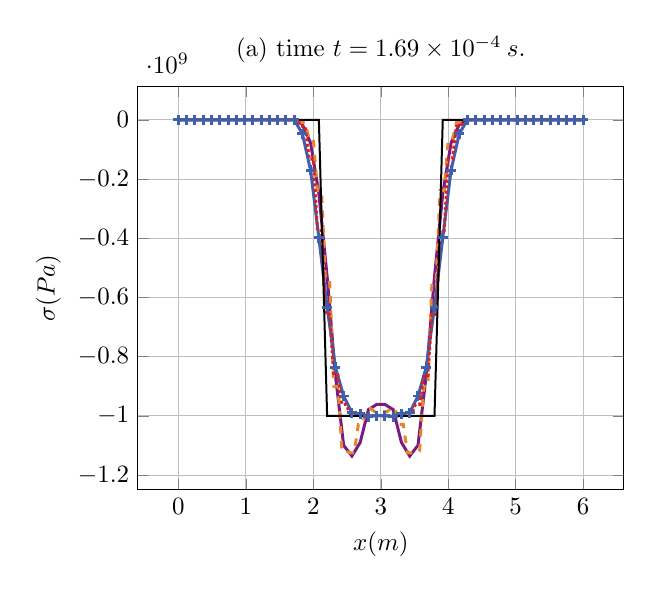
\begin{tikzpicture}[scale=0.9]
\begin{axis}[xlabel=$x (m)$,ylabel=$\sigma (Pa)$,ymajorgrids=true,xmajorgrids=true,title={(a) time $t=1.69\times 10^{-4}\: s.$}]
\addplot[Purple,very thick,mark=none,solid] coordinates {(0.0,-9.62200780097e-08) (0.122448979592,-1.92440156019e-07) (0.244897959184,-9.62200780097e-08) (0.367346938776,0.0) (0.489795918367,9.62200780097e-08) (0.612244897959,-9.62200780097e-08) (0.734693877551,-1.92440156019e-07) (0.857142857143,-9.62200780097e-08) (0.979591836735,-9.62200780097e-08) (1.10204081633,0.0) (1.22448979592,9.62200780097e-08) (1.34693877551,-9.62200780097e-08) (1.4693877551,0.0) (1.59183673469,0.0) (1.71428571429,0.0) (1.83673469388,-15437652.4848) (1.95918367347,-78183137.9185) (2.08163265306,-249067223.585) (2.20408163265,-529536815.675) (2.32653061224,-862202048.46) (2.44897959184,-1099498863.41) (2.57142857143,-1135789315.44) (2.69387755102,-1090007223.73) (2.81632653061,-978780358.738) (2.9387755102,-961497360.562) (3.0612244898,-961497360.562) (3.18367346939,-978780358.738) (3.30612244898,-1090007223.73) (3.42857142857,-1135789315.44) (3.55102040816,-1099498863.41) (3.67346938776,-862202048.46) (3.79591836735,-529536815.675) (3.91836734694,-249067223.585) (4.04081632653,-78183137.9185) (4.16326530612,-15437652.4848) (4.28571428571,-3.85185988877e-23) (4.40816326531,-9.62200780097e-08) (4.5306122449,9.62200780097e-08) (4.65306122449,9.62200780097e-08) (4.77551020408,9.62200780097e-08) (4.89795918367,-2.88660234029e-07) (5.02040816327,-9.62200780097e-08) (5.14285714286,9.62200780097e-08) (5.26530612245,1.92440156019e-07) (5.38775510204,2.88660234029e-07) (5.51020408163,9.62200780097e-08) (5.63265306122,0.0) (5.75510204082,0.0) (5.87755102041,0.0) (6.0,-9.62200780097e-08) };
\addplot[Orange,very thick,mark=none,dashed] coordinates {(0.0,0.0) (0.0606060606061,0.0) (0.121212121212,9.52481580298e-08) (0.181818181818,9.52481580298e-08) (0.242424242424,9.52481580298e-08) (0.30303030303,9.52481580298e-08) (0.363636363636,0.0) (0.424242424242,0.0) (0.484848484848,-9.52481580298e-08) (0.545454545455,-9.52481580298e-08) (0.606060606061,-1.9049631606e-07) (0.666666666667,-1.9049631606e-07) (0.727272727273,0.0) (0.787878787879,0.0) (0.848484848485,0.0) (0.909090909091,0.0) (0.969696969697,-3.85185988877e-23) (1.0303030303,-3.85185988877e-23) (1.09090909091,-9.52481580298e-08) (1.15151515152,-9.52481580298e-08) (1.21212121212,9.52481580298e-08) (1.27272727273,9.52481580298e-08) (1.33333333333,9.52481580298e-08) (1.39393939394,9.52481580298e-08) (1.45454545455,-1.9049631606e-07) (1.51515151515,-1.9049631606e-07) (1.57575757576,1.9049631606e-07) (1.63636363636,1.9049631606e-07) (1.69696969697,0.0) (1.75757575758,0.0) (1.81818181818,-9533923.2537) (1.87878787879,-9533923.2537) (1.93939393939,-67166647.336) (2.0,-67166647.336) (2.06060606061,-239339979.822) (2.12121212121,-239339979.822) (2.18181818182,-549695480.518) (2.24242424242,-549695480.518) (2.30303030303,-900240202.504) (2.36363636364,-900240202.504) (2.42424242424,-1118552245.0) (2.48484848485,-1118552245.0) (2.54545454545,-1125362633.2) (2.60606060606,-1125362633.2) (2.66666666667,-1028724363.35) (2.72727272727,-1028724363.35) (2.78787878788,-975375246.836) (2.84848484848,-975375246.836) (2.90909090909,-986009278.185) (2.9696969697,-986009278.185) (3.0303030303,-986009278.185) (3.09090909091,-986009278.185) (3.15151515152,-975375246.836) (3.21212121212,-975375246.836) (3.27272727273,-1028724363.35) (3.33333333333,-1028724363.35) (3.39393939394,-1125362633.2) (3.45454545455,-1125362633.2) (3.51515151515,-1118552245.0) (3.57575757576,-1118552245.0) (3.63636363636,-900240202.504) (3.69696969697,-900240202.504) (3.75757575758,-549695480.518) (3.81818181818,-549695480.518) (3.87878787879,-239339979.822) (3.93939393939,-239339979.822) (4.0,-67166647.336) (4.06060606061,-67166647.336) (4.12121212121,-9533923.2537) (4.18181818182,-9533923.2537) (4.24242424242,9.52481580298e-08) (4.30303030303,9.52481580298e-08) (4.36363636364,-9.52481580298e-08) (4.42424242424,-9.52481580298e-08) (4.48484848485,0.0) (4.54545454545,0.0) (4.60606060606,0.0) (4.66666666667,0.0) (4.72727272727,0.0) (4.78787878788,0.0) (4.84848484848,0.0) (4.90909090909,0.0) (4.9696969697,0.0) (5.0303030303,0.0) (5.09090909091,0.0) (5.15151515152,0.0) (5.21212121212,0.0) (5.27272727273,0.0) (5.33333333333,0.0) (5.39393939394,0.0) (5.45454545455,0.0) (5.51515151515,0.0) (5.57575757576,0.0) (5.63636363636,0.0) (5.69696969697,0.0) (5.75757575758,0.0) (5.81818181818,0.0) (5.87878787879,0.0) (5.93939393939,9.52481580298e-08) (6.0,9.52481580298e-08) };
\addplot[Blue,very thick,mark=+,solid] coordinates {(0.0,9.62200780097e-08) (0.122448979592,1.92440156019e-07) (0.244897959184,-2.88660234029e-07) (0.367346938776,-1.92440156019e-07) (0.489795918367,-9.62200780097e-08) (0.612244897959,-1.92440156019e-07) (0.734693877551,-3.84880312039e-07) (0.857142857143,-1.92440156019e-07) (0.979591836735,-9.62200780097e-08) (1.10204081633,0.0) (1.22448979592,9.62200780097e-08) (1.34693877551,-9.62200780097e-08) (1.4693877551,0.0) (1.59183673469,0.0) (1.71428571429,0.0) (1.83673469388,-46578287.5426) (1.95918367347,-171036560.611) (2.08163265306,-398499931.778) (2.20408163265,-632823078.817) (2.32653061224,-835128021.529) (2.44897959184,-932849760.398) (2.57142857143,-988852888.782) (2.69387755102,-992828858.011) (2.81632653061,-1002356300.0) (2.9387755102,-999046312.534) (3.0612244898,-999046312.534) (3.18367346939,-1002356300.0) (3.30612244898,-992828858.011) (3.42857142857,-988852888.782) (3.55102040816,-932849760.398) (3.67346938776,-835128021.529) (3.79591836735,-632823078.817) (3.91836734694,-398499931.778) (4.04081632653,-171036560.611) (4.16326530612,-46578287.5426) (4.28571428571,0.0) (4.40816326531,-9.62200780097e-08) (4.5306122449,-1.92592994439e-23) (4.65306122449,1.92440156019e-07) (4.77551020408,0.0) (4.89795918367,-9.62200780097e-08) (5.02040816327,0.0) (5.14285714286,0.0) (5.26530612245,3.85185988877e-23) (5.38775510204,1.92440156019e-07) (5.51020408163,9.62200780097e-08) (5.63265306122,0.0) (5.75510204082,9.62200780097e-08) (5.87755102041,0.0) (6.0,-9.62200780097e-08) };
\addplot[Red,very thick,mark=none,densely dotted] coordinates {(0.0,-1.9049631606e-07) (0.0606060606061,-1.9049631606e-07) (0.121212121212,0.0) (0.181818181818,0.0) (0.242424242424,9.52481580298e-08) (0.30303030303,9.52481580298e-08) (0.363636363636,-9.52481580298e-08) (0.424242424242,-9.52481580298e-08) (0.484848484848,-1.9049631606e-07) (0.545454545455,-1.9049631606e-07) (0.606060606061,0.0) (0.666666666667,0.0) (0.727272727273,0.0) (0.787878787879,0.0) (0.848484848485,0.0) (0.909090909091,0.0) (0.969696969697,-9.52481580298e-08) (1.0303030303,-9.52481580298e-08) (1.09090909091,-1.9049631606e-07) (1.15151515152,-1.9049631606e-07) (1.21212121212,-9.52481580298e-08) (1.27272727273,-9.52481580298e-08) (1.33333333333,0.0) (1.39393939394,0.0) (1.45454545455,9.52481580298e-08) (1.51515151515,9.52481580298e-08) (1.57575757576,-9.52481580298e-08) (1.63636363636,-9.52481580298e-08) (1.69696969697,0.0) (1.75757575758,0.0) (1.81818181818,-21051436.477) (1.87878787879,-21051436.477) (1.93939393939,-132631129.917) (2.0,-132631129.917) (2.06060606061,-373920143.932) (2.12121212121,-373920143.932) (2.18181818182,-657449507.004) (2.24242424242,-657449507.004) (2.30303030303,-862932918.65) (2.36363636364,-862932918.65) (2.42424242424,-960874193.44) (2.48484848485,-960874193.44) (2.54545454545,-992227161.455) (2.60606060606,-992227161.455) (2.66666666667,-998999192.727) (2.72727272727,-998999192.727) (2.78787878788,-999914743.293) (2.84848484848,-999914743.293) (2.90909090909,-999999573.105) (2.9696969697,-999999573.105) (3.0303030303,-999999573.105) (3.09090909091,-999999573.105) (3.15151515152,-999914743.293) (3.21212121212,-999914743.293) (3.27272727273,-998999192.727) (3.33333333333,-998999192.727) (3.39393939394,-992227161.455) (3.45454545455,-992227161.455) (3.51515151515,-960874193.44) (3.57575757576,-960874193.44) (3.63636363636,-862932918.65) (3.69696969697,-862932918.65) (3.75757575758,-657449507.004) (3.81818181818,-657449507.004) (3.87878787879,-373920143.932) (3.93939393939,-373920143.932) (4.0,-132631129.917) (4.06060606061,-132631129.917) (4.12121212121,-21051436.477) (4.18181818182,-21051436.477) (4.24242424242,-9.52481580298e-08) (4.30303030303,-9.52481580298e-08) (4.36363636364,9.52481580298e-08) (4.42424242424,9.52481580298e-08) (4.48484848485,0.0) (4.54545454545,0.0) (4.60606060606,0.0) (4.66666666667,0.0) (4.72727272727,0.0) (4.78787878788,0.0) (4.84848484848,0.0) (4.90909090909,0.0) (4.9696969697,0.0) (5.0303030303,0.0) (5.09090909091,0.0) (5.15151515152,0.0) (5.21212121212,0.0) (5.27272727273,0.0) (5.33333333333,0.0) (5.39393939394,0.0) (5.45454545455,0.0) (5.51515151515,0.0) (5.57575757576,0.0) (5.63636363636,0.0) (5.69696969697,0.0) (5.75757575758,0.0) (5.81818181818,0.0) (5.87878787879,0.0) (5.93939393939,-1.9049631606e-07) (6.0,-1.9049631606e-07) };
\addplot[black,thick] coordinates {(0.0,-0.0) (0.122448979592,-0.0) (0.244897959184,-0.0) (0.367346938776,-0.0) (0.489795918367,-0.0) (0.612244897959,-0.0) (0.734693877551,-0.0) (0.857142857143,-0.0) (0.979591836735,-0.0) (1.10204081633,-0.0) (1.22448979592,-0.0) (1.34693877551,-0.0) (1.4693877551,-0.0) (1.59183673469,-0.0) (1.71428571429,-0.0) (1.83673469388,-0.0) (1.95918367347,-0.0) (2.08163265306,-0.0) (2.20408163265,-1000000000.0) (2.32653061224,-1000000000.0) (2.44897959184,-1000000000.0) (2.57142857143,-1000000000.0) (2.69387755102,-1000000000.0) (2.81632653061,-1000000000.0) (2.9387755102,-1000000000.0) (3.0612244898,-1000000000.0) (3.18367346939,-1000000000.0) (3.30612244898,-1000000000.0) (3.42857142857,-1000000000.0) (3.55102040816,-1000000000.0) (3.67346938776,-1000000000.0) (3.79591836735,-1000000000.0) (3.91836734694,-0.0) (4.04081632653,-0.0) (4.16326530612,-0.0) (4.28571428571,-0.0) (4.40816326531,-0.0) (4.5306122449,-0.0) (4.65306122449,-0.0) (4.77551020408,-0.0) (4.89795918367,-0.0) (5.02040816327,-0.0) (5.14285714286,-0.0) (5.26530612245,-0.0) (5.38775510204,-0.0) (5.51020408163,-0.0) (5.63265306122,-0.0) (5.75510204082,-0.0) (5.87755102041,-0.0) (6.0,-0.0) };
%\legend{mpm 1ppc,mpm 2ppc,modmpm 1ppc,modmpm 2ppc}
\end{axis}
\end{tikzpicture}
 \phantomsubcaption \label{subfig:mpm_diffusion_10}}
  {\definecolor{Purple}{RGB}{120,28,129}
\definecolor{Orange}{RGB}{231,133,50}
\definecolor{Blue}{RGB}{63,96,174}
\definecolor{Red}{RGB}{217,33,32}
\definecolor{Duck}{RGB}{83,158,182}
\definecolor{Green}{RGB}{109,179,136}
\definecolor{Yellow}{RGB}{202,184,67}
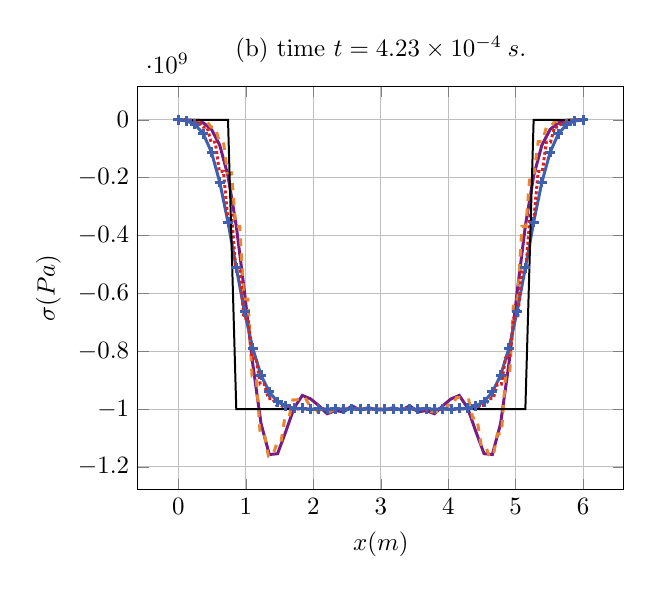
\begin{tikzpicture}[scale=0.9]
\begin{axis}[xlabel=$x (m)$,ylabel=$\sigma (Pa)$,ymajorgrids=true,xmajorgrids=true,title={(b) time $t=4.23\times 10^{-4}\: s.$}]
\addplot[Purple,very thick,mark=none,solid] coordinates {(0.0,-39934.2174897) (0.122448979592,-406302.064953) (0.244897959184,-2420460.88495) (0.367346938776,-10136844.8366) (0.489795918367,-33063216.5915) (0.612244897959,-87547121.3685) (0.734693877551,-194171704.565) (0.857142857143,-366493404.576) (0.979591836735,-596875114.898) (1.10204081633,-845116689.368) (1.22448979592,-1050481005.19) (1.34693877551,-1157297307.0) (1.4693877551,-1154376682.02) (1.59183673469,-1077374033.62) (1.71428571429,-995689036.388) (1.83673469388,-952936697.469) (1.95918367347,-964832377.273) (2.08163265306,-988568067.368) (2.20408163265,-1016260759.09) (2.32653061224,-1005179173.62) (2.44897959184,-1009892551.13) (2.57142857143,-988773783.034) (2.69387755102,-1003829596.99) (2.81632653061,-995025027.704) (2.9387755102,-1003213108.71) (3.0612244898,-1003213108.71) (3.18367346939,-995025027.704) (3.30612244898,-1003829596.99) (3.42857142857,-988773783.034) (3.55102040816,-1009892551.13) (3.67346938776,-1005179173.62) (3.79591836735,-1016260759.09) (3.91836734694,-988568067.368) (4.04081632653,-964832377.273) (4.16326530612,-952936697.469) (4.28571428571,-995689036.388) (4.40816326531,-1077374033.62) (4.5306122449,-1154376682.02) (4.65306122449,-1157297307.0) (4.77551020408,-1050481005.19) (4.89795918367,-845116689.368) (5.02040816327,-596875114.898) (5.14285714286,-366493404.576) (5.26530612245,-194171704.565) (5.38775510204,-87547121.3685) (5.51020408163,-33063216.5915) (5.63265306122,-10136844.8366) (5.75510204082,-2420460.88495) (5.87755102041,-406302.064953) (6.0,-39934.2174897) };
\addplot[Orange,very thick,mark=none,dashed] coordinates {(0.0,-10429.0753611) (0.0606060606061,-10429.0753611) (0.121212121212,-161982.808053) (0.181818181818,-161982.808053) (0.242424242424,-1267409.75703) (0.30303030303,-1267409.75703) (0.363636363636,-6575307.60772) (0.424242424242,-6575307.60772) (0.484848484848,-25213047.7874) (0.545454545455,-25213047.7874) (0.606060606061,-75630068.1866) (0.666666666667,-75630068.1866) (0.727272727273,-183565723.323) (0.787878787879,-183565723.323) (0.848484848485,-368376215.18) (0.909090909091,-368376215.18) (0.969696969697,-620238104.743) (1.0303030303,-620238104.743) (1.09090909091,-886041263.042) (1.15151515152,-886041263.042) (1.21212121212,-1086232263.3) (1.27272727273,-1086232263.3) (1.33333333333,-1162610811.08) (1.39393939394,-1162610811.08) (1.45454545455,-1121800356.23) (1.51515151515,-1121800356.23) (1.57575757576,-1031608883.18) (1.63636363636,-1031608883.18) (1.69696969697,-967968470.151) (1.75757575758,-967968470.151) (1.81818181818,-960540680.349) (1.87878787879,-960540680.349) (1.93939393939,-986227377.719) (2.0,-986227377.719) (2.06060606061,-1007602191.25) (2.12121212121,-1007602191.25) (2.18181818182,-1009726046.8) (2.24242424242,-1009726046.8) (2.30303030303,-1002072997.71) (2.36363636364,-1002072997.71) (2.42424242424,-997465464.463) (2.48484848485,-997465464.463) (2.54545454545,-998318352.653) (2.60606060606,-998318352.653) (2.66666666667,-1000280134.99) (2.72727272727,-1000280134.99) (2.78787878788,-1000550813.71) (2.84848484848,-1000550813.71) (2.90909090909,-999915604.91) (2.9696969697,-999915604.91) (3.0303030303,-999915604.91) (3.09090909091,-999915604.91) (3.15151515152,-1000550813.71) (3.21212121212,-1000550813.71) (3.27272727273,-1000280134.99) (3.33333333333,-1000280134.99) (3.39393939394,-998318352.653) (3.45454545455,-998318352.653) (3.51515151515,-997465464.463) (3.57575757576,-997465464.463) (3.63636363636,-1002072997.71) (3.69696969697,-1002072997.71) (3.75757575758,-1009726046.8) (3.81818181818,-1009726046.8) (3.87878787879,-1007602191.25) (3.93939393939,-1007602191.25) (4.0,-986227377.719) (4.06060606061,-986227377.719) (4.12121212121,-960540680.349) (4.18181818182,-960540680.349) (4.24242424242,-967968470.151) (4.30303030303,-967968470.151) (4.36363636364,-1031608883.18) (4.42424242424,-1031608883.18) (4.48484848485,-1121800356.23) (4.54545454545,-1121800356.23) (4.60606060606,-1162610811.08) (4.66666666667,-1162610811.08) (4.72727272727,-1086232263.3) (4.78787878788,-1086232263.3) (4.84848484848,-886041263.042) (4.90909090909,-886041263.042) (4.9696969697,-620238104.743) (5.0303030303,-620238104.743) (5.09090909091,-368376215.18) (5.15151515152,-368376215.18) (5.21212121212,-183565723.323) (5.27272727273,-183565723.323) (5.33333333333,-75630068.1866) (5.39393939394,-75630068.1866) (5.45454545455,-25213047.7874) (5.51515151515,-25213047.7874) (5.57575757576,-6575307.60772) (5.63636363636,-6575307.60772) (5.69696969697,-1267409.75703) (5.75757575758,-1267409.75703) (5.81818181818,-161982.808054) (5.87878787879,-161982.808054) (5.93939393939,-10429.0753609) (6.0,-10429.0753609) };
\addplot[Blue,very thick,mark=+,solid] coordinates {(0.0,-508931.478279) (0.122448979592,-3748025.68591) (0.244897959184,-16014385.4746) (0.367346938776,-47881742.3505) (0.489795918367,-112174746.169) (0.612244897959,-215592738.441) (0.734693877551,-354671855.848) (0.857142857143,-511212799.02) (0.979591836735,-663838312.129) (1.10204081633,-790213464.162) (1.22448979592,-883647482.448) (1.34693877551,-941000619.105) (1.4693877551,-974959939.111) (1.59183673469,-988927861.484) (1.71428571429,-997557909.852) (1.83673469388,-997805889.972) (1.95918367347,-1000931915.66) (2.08163265306,-998709339.041) (2.20408163265,-1001197182.01) (2.32653061224,-998859728.815) (2.44897959184,-1001017871.89) (2.57142857143,-999150004.014) (2.69387755102,-1000640138.33) (2.81632653061,-999602146.851) (2.9387755102,-1000134970.66) (3.0612244898,-1000134970.66) (3.18367346939,-999602146.851) (3.30612244898,-1000640138.33) (3.42857142857,-999150004.014) (3.55102040816,-1001017871.89) (3.67346938776,-998859728.815) (3.79591836735,-1001197182.01) (3.91836734694,-998709339.041) (4.04081632653,-1000931915.66) (4.16326530612,-997805889.972) (4.28571428571,-997557909.852) (4.40816326531,-988927861.484) (4.5306122449,-974959939.111) (4.65306122449,-941000619.105) (4.77551020408,-883647482.448) (4.89795918367,-790213464.162) (5.02040816327,-663838312.129) (5.14285714286,-511212799.02) (5.26530612245,-354671855.848) (5.38775510204,-215592738.441) (5.51020408163,-112174746.169) (5.63265306122,-47881742.3505) (5.75510204082,-16014385.4746) (5.87755102041,-3748025.68591) (6.0,-508931.478279) };
\addplot[Red,very thick,mark=none,densely dotted] coordinates {(0.0,-61223.9335744) (0.0606060606061,-61223.9335744) (0.121212121212,-884894.710625) (0.181818181818,-884894.710625) (0.242424242424,-6003361.51961) (0.30303030303,-6003361.51961) (0.363636363636,-25575128.3809) (0.424242424242,-25575128.3809) (0.484848484848,-77365275.2782) (0.545454545455,-77365275.2782) (0.606060606061,-178548645.631) (0.666666666667,-178548645.631) (0.727272727273,-330659471.659) (0.787878787879,-330659471.659) (0.848484848485,-511731335.491) (0.909090909091,-511731335.491) (0.969696969697,-686005012.829) (1.0303030303,-686005012.829) (1.09090909091,-823733433.992) (1.15151515152,-823733433.992) (1.21212121212,-914145742.521) (1.27272727273,-914145742.521) (1.33333333333,-963861687.734) (1.39393939394,-963861687.734) (1.45454545455,-986895334.229) (1.51515151515,-986895334.229) (1.57575757576,-995919063.725) (1.63636363636,-995919063.725) (1.69696969697,-998912836.991) (1.75757575758,-998912836.991) (1.81818181818,-999753499.27) (1.87878787879,-999753499.27) (1.93939393939,-999952757.55) (2.0,-999952757.55) (2.06060606061,-999992418.488) (2.12121212121,-999992418.488) (2.18181818182,-999998994.239) (2.24242424242,-999998994.239) (2.30303030303,-999999891.711) (2.36363636364,-999999891.711) (2.42424242424,-999999990.727) (2.48484848485,-999999990.727) (2.54545454545,-999999999.438) (2.60606060606,-999999999.438) (2.66666666667,-999999999.942) (2.72727272727,-999999999.942) (2.78787878788,-1000000000.02) (2.84848484848,-1000000000.02) (2.90909090909,-999999999.993) (2.9696969697,-999999999.993) (3.0303030303,-999999999.993) (3.09090909091,-999999999.993) (3.15151515152,-1000000000.02) (3.21212121212,-1000000000.02) (3.27272727273,-999999999.942) (3.33333333333,-999999999.942) (3.39393939394,-999999999.438) (3.45454545455,-999999999.438) (3.51515151515,-999999990.727) (3.57575757576,-999999990.727) (3.63636363636,-999999891.711) (3.69696969697,-999999891.711) (3.75757575758,-999998994.239) (3.81818181818,-999998994.239) (3.87878787879,-999992418.488) (3.93939393939,-999992418.488) (4.0,-999952757.55) (4.06060606061,-999952757.55) (4.12121212121,-999753499.27) (4.18181818182,-999753499.27) (4.24242424242,-998912836.991) (4.30303030303,-998912836.991) (4.36363636364,-995919063.725) (4.42424242424,-995919063.725) (4.48484848485,-986895334.229) (4.54545454545,-986895334.229) (4.60606060606,-963861687.734) (4.66666666667,-963861687.734) (4.72727272727,-914145742.521) (4.78787878788,-914145742.521) (4.84848484848,-823733433.992) (4.90909090909,-823733433.992) (4.9696969697,-686005012.829) (5.0303030303,-686005012.829) (5.09090909091,-511731335.491) (5.15151515152,-511731335.491) (5.21212121212,-330659471.659) (5.27272727273,-330659471.659) (5.33333333333,-178548645.631) (5.39393939394,-178548645.631) (5.45454545455,-77365275.2782) (5.51515151515,-77365275.2782) (5.57575757576,-25575128.3809) (5.63636363636,-25575128.3809) (5.69696969697,-6003361.51961) (5.75757575758,-6003361.51961) (5.81818181818,-884894.710625) (5.87878787879,-884894.710625) (5.93939393939,-61223.9335744) (6.0,-61223.9335744) };
\addplot[black,thick] coordinates {(0.0,-0.0) (0.122448979592,-0.0) (0.244897959184,-0.0) (0.367346938776,-0.0) (0.489795918367,-0.0) (0.612244897959,-0.0) (0.734693877551,-0.0) (0.857142857143,-1000000000.0) (0.979591836735,-1000000000.0) (1.10204081633,-1000000000.0) (1.22448979592,-1000000000.0) (1.34693877551,-1000000000.0) (1.4693877551,-1000000000.0) (1.59183673469,-1000000000.0) (1.71428571429,-1000000000.0) (1.83673469388,-1000000000.0) (1.95918367347,-1000000000.0) (2.08163265306,-1000000000.0) (2.20408163265,-1000000000.0) (2.32653061224,-1000000000.0) (2.44897959184,-1000000000.0) (2.57142857143,-1000000000.0) (2.69387755102,-1000000000.0) (2.81632653061,-1000000000.0) (2.9387755102,-1000000000.0) (3.0612244898,-1000000000.0) (3.18367346939,-1000000000.0) (3.30612244898,-1000000000.0) (3.42857142857,-1000000000.0) (3.55102040816,-1000000000.0) (3.67346938776,-1000000000.0) (3.79591836735,-1000000000.0) (3.91836734694,-1000000000.0) (4.04081632653,-1000000000.0) (4.16326530612,-1000000000.0) (4.28571428571,-1000000000.0) (4.40816326531,-1000000000.0) (4.5306122449,-1000000000.0) (4.65306122449,-1000000000.0) (4.77551020408,-1000000000.0) (4.89795918367,-1000000000.0) (5.02040816327,-1000000000.0) (5.14285714286,-1000000000.0) (5.26530612245,-0.0) (5.38775510204,-0.0) (5.51020408163,-0.0) (5.63265306122,-0.0) (5.75510204082,-0.0) (5.87755102041,-0.0) (6.0,-0.0) };
%\legend{mpm 1ppc,mpm 2ppc,modmpm 1ppc,modmpm 2ppc}
\end{axis}
\end{tikzpicture}
 \phantomsubcaption \label{subfig:mpm_diffusion_25}}
  {\definecolor{Purple}{RGB}{120,28,129}
\definecolor{Orange}{RGB}{231,133,50}
\definecolor{Blue}{RGB}{63,96,174}
\definecolor{Red}{RGB}{217,33,32}
\definecolor{Duck}{RGB}{83,158,182}
\definecolor{Green}{RGB}{109,179,136}
\definecolor{Yellow}{RGB}{202,184,67}
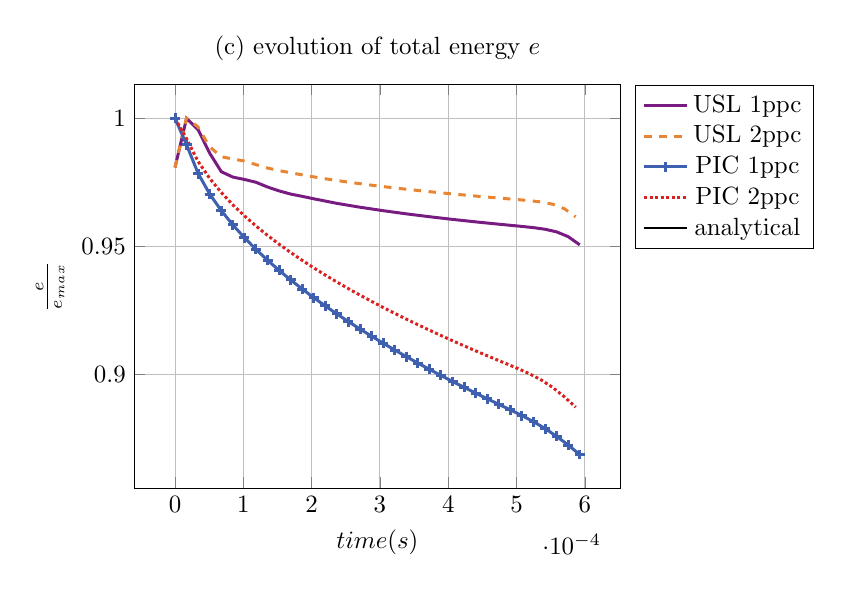
\begin{tikzpicture}[scale=0.9]
\begin{axis}[xlabel=$time (s)$,ylabel=$\frac{e}{e_{max}}$,ymajorgrids=true,xmajorgrids=true,title={(c) evolution of total energy $e$}, legend pos=outer north east]
\addplot[Purple,very thick,mark=none,solid] coordinates {(0.0,0.980776775206) (1.69272151355e-05,1.0) (3.38544302711e-05,0.995486386818) (5.07816454066e-05,0.986335480918) (6.77088605422e-05,0.979118179787) (8.46360756777e-05,0.977011836735) (0.000101563290813,0.976083552705) (0.000118490505949,0.974985958077) (0.000135417721084,0.973132007483) (0.00015234493622,0.971614043952) (0.000169272151355,0.970370597838) (0.000186199366491,0.969484052645) (0.000203126581626,0.968527091175) (0.000220053796762,0.967645365047) (0.000236981011898,0.966743210911) (0.000253908227033,0.965982183586) (0.000270835442169,0.965231974397) (0.000287762657304,0.964563191524) (0.00030468987244,0.96388114719) (0.000321617087575,0.963263530823) (0.000338544302711,0.962646353557) (0.000355471517846,0.962084695394) (0.000372398732982,0.961521764293) (0.000389325948117,0.961001071279) (0.000406253163253,0.960479919884) (0.000423180378389,0.959994795728) (0.000440107593524,0.959510651477) (0.00045703480866,0.959056403386) (0.000473962023795,0.958603029859) (0.000490889238931,0.958172736022) (0.000507816454066,0.957731808745) (0.000524743669202,0.957261239502) (0.000541670884337,0.956629022745) (0.000558598099473,0.95560284594) (0.000575525314608,0.953743784185) (0.000592452529744,0.950544066664) };
\addplot[Orange,very thick,mark=none,dashed] coordinates {(0.0,0.980776775206) (1.67562331645e-05,1.0) (3.3512466329e-05,0.996663809337) (5.02686994934e-05,0.98900666995) (6.70249326579e-05,0.985020324447) (8.37811658224e-05,0.984110580813) (0.000100537398987,0.983326915208) (0.000117293632151,0.981979184866) (0.000134049865316,0.980638155666) (0.00015080609848,0.979617302856) (0.000167562331645,0.978778886884) (0.000184318564809,0.977968446843) (0.000201074797974,0.977176694993) (0.000217831031138,0.976440965591) (0.000234587264303,0.975764557777) (0.000251343497467,0.975128766754) (0.000268099730632,0.974522184343) (0.000284855963796,0.973943735564) (0.000301612196961,0.973393220953) (0.000318368430125,0.972867749193) (0.00033512466329,0.972363947434) (0.000351880896454,0.971879647077) (0.000368637129618,0.971413467384) (0.000385393362783,0.970964070517) (0.000402149595947,0.97053007437) (0.000418905829112,0.970110254428) (0.000435662062276,0.969703595912) (0.000452418295441,0.969309210173) (0.000469174528605,0.96892621672) (0.00048593076177,0.968553101725) (0.000502686994934,0.968183689821) (0.000519443228099,0.96779053395) (0.000536199461263,0.967278784767) (0.000552955694428,0.96640240077) (0.000569711927592,0.964686590438) (0.000586468160757,0.961481917033) };
\addplot[Blue,very thick,mark=+,solid] coordinates {(0.0,1.0) (1.69272151355e-05,0.9896) (3.38544302711e-05,0.97840192) (5.07816454066e-05,0.970395814144) (6.77088605422e-05,0.963922377931) (8.46360756777e-05,0.958330092512) (0.000101563290813,0.953327939993) (0.000118490505949,0.948758714644) (0.000135417721084,0.944525461648) (0.00015234493622,0.940563061208) (0.000169272151355,0.936825160363) (0.000186199366491,0.933277336034) (0.000203126581626,0.929893178182) (0.000220053796762,0.926651891851) (0.000236981011898,0.923536752237) (0.000253908227033,0.92053406787) (0.000270835442169,0.917632461061) (0.000287762657304,0.914822354268) (0.00030468987244,0.912095594541) (0.000321617087575,0.909445173164) (0.000338544302711,0.906865012545) (0.000355471517846,0.904349801607) (0.000372398732982,0.901894866831) (0.000389325948117,0.899496069935) (0.000406253163253,0.897149725755) (0.000423180378389,0.894852535658) (0.000440107593524,0.892601494491) (0.00045703480866,0.890393110082) (0.000473962023795,0.888218874172) (0.000490889238931,0.886052220178) (0.000507816454066,0.883829497068) (0.000524743669202,0.881442958718) (0.000541670884337,0.878767030396) (0.000558598099473,0.875715616111) (0.000575525314608,0.872297097702) (0.000592452529744,0.868628627691) };
\addplot[Red,very thick,mark=none,densely dotted] coordinates {(0.0,1.0) (1.67562331645e-05,0.9921) (3.3512466329e-05,0.98321470125) (5.02686994934e-05,0.976674798128) (6.70249326579e-05,0.971199634535) (8.37811658224e-05,0.966410687731) (0.000100537398987,0.962109118378) (0.000117293632151,0.958172229577) (0.000134049865316,0.954520707917) (0.00015080609848,0.951100328411) (0.000167562331645,0.947872098186) (0.000184318564809,0.944806876372) (0.000201074797974,0.941882214857) (0.000217831031138,0.939080387869) (0.000234587264303,0.936387108509) (0.000251343497467,0.933790661554) (0.000268099730632,0.931281298637) (0.000284855963796,0.928850804847) (0.000301612196961,0.926492180888) (0.000318368430125,0.924199405234) (0.00033512466329,0.92196725296) (0.000351880896454,0.919791155586) (0.000368637129618,0.917667091102) (0.000385393362783,0.915591496621) (0.000402149595947,0.913561198187) (0.000418905829112,0.911573353815) (0.000435662062276,0.909625405615) (0.000452418295441,0.907714970883) (0.000469174528605,0.905838699657) (0.00048593076177,0.903984815557) (0.000502686994934,0.902108349787) (0.000519443228099,0.900090874846) (0.000536199461263,0.89772781162) (0.000552955694428,0.894800303924) (0.000569711927592,0.891215939989) (0.000586468160757,0.8871100207) };
\addplot[black,thick] coordinates {(0.,1.) (0.0000001,1.)};
\legend{USL 1ppc,USL 2ppc,PIC 1ppc,PIC 2ppc,analytical}
\end{axis}
\end{tikzpicture}

%%% Local Variables: 
%%% mode: latex
%%% TeX-master: "../../mainManuscript"
%%% End:
 \phantomsubcaption \label{subfig:mpm_energies}}
  \caption{Comparison of USL solutions using either PIC or FLIP projection and exact solution of the bars impact problem for various discretizations. (a)--(b) comparison of stress profiles at several time steps (c) evolution of total energy. Parameters: $CFL=0.7$ ; $v_0=\frac{1}{200}\sqrt{\frac{E}{\rho}}$.}
  \label{fig:mpm_diffusion}
\end{figure}
As can be seen, PIC projection eliminates the noise in numerical solutions as well as the velocity locking in the central region of the bar. In addition, stress results provided by the USL using PIC mapping are also close to the exact solution (see figures \ref{fig:mpm_diffusion}\subref{subfig:mpm_diffusion_10} and \ref{fig:mpm_diffusion}\subref{subfig:mpm_diffusion_25}). However, the resolution of discontinuities allowed by the "modified" USL--MPM is slightly lower than that of the original formulation owing to numerical diffusion as shown in the energy plot in figure \ref{fig:mpm_diffusion}\subref{subfig:mpm_energies}. This result was expected since the FLIP projection was preferred to PIC one for it enabled a reduction of numerical dissipation \cite{PIC_Nishiguchi}.

% This balance between diffusion and noise resulting from the projection between nodes and particles selected has been emphasized in \cite{XPIC}
% Furthermore, the mapping \eqref{eq:PIC_Back-mapping} has been identified in \cite{XPIC} as a solution of the problem:
% \begin{equation}
%   \vect{v}^{p,n+1} = \arg \min_{\vect{v}^{p}}|| \vect{v}^{p}||_2,\quad \text{such that }  \frac{\sum_{p=1}^{N_p}S_{ip} m_p\vect{v}^{p}}{\sum_{k=1}^{N_p}S_{ik} m_k}=\vect{v}^{i,n+1}
% \end{equation}
% in which the minimization is achieved by dissipating kinetic energy.
 
\subsection{Strategy for reducing oscillations and diffusion}
We are concerned here with the accurate solution of hyperbolic problems in solid undergoing finite deformations. Although the MPM enables an efficient management of large strains, the oscillations it suffers from do not allow to accurately capture waves propagating in a medium. The above numerical simulations however suggest that noise can be removed by using an interpolation instead of an update of material points velocity, at the cost of additional diffusion. Thus, the use of  a linear combination of PIC and FLIP projections to update particles velocity was proposed in \cite{Nairn}, which can be seen as an artificial damping. Further, a tunable mapping procedure based on a parameter $m$ that completely eliminates noise in MPM solution has been proposed in the \textit{Extended PIC of order m (XPIC(m))} \cite{XPIC}. A classical interpolation is selected for $m=1$ whereas the mapping tends to FLIP one as $m \rightarrow \infty$ while avoiding oscillations in dissipating energy. Therefore, the method is still unable to capture discontinuities.

The point of view adopted in this thesis is that numerical diffusion is essentially due to the projection of fields from nodes to particles which spreads the information. Hence, a reduction of the domain of influence of nodes might result in lower dissipation. As a consequence, the reintroduction of PIC mapping combined to the \textit{Discontinuous Galerkin} approximation (DG) within the MPM is proposed here. These two features are expected to respectively avoid spurious oscillations and limit numerical diffusion.


%%% Local Variables: 
%%% mode: latex
%%% TeX-master: "../mainManuscript"
%%% End:
